\documentclass[cjk,slidestop,compress,mathserif,blue]{beamer}
%dvipdfm选项是关键,否则编译统统通不过
%beamer的颜色选项定义的是导航条和标题的颜色(即关键词structure的颜色)

%%%%%%%%%%%%%%%%仅限于XeTeX可使用的宏包%%%%%%%%%%%%%%%%%%%%%%%%%%%%
\usepackage{fontspec,xunicode,xltxtra,beamerthemesplit}
%\usepackage{beamerthemesplit}
\usepackage{xeCJK}
\setCJKmainfont[BoldFont=黑体, ItalicFont=楷体, BoldItalicFont=仿宋]{黑体}
%\setsansfont[Mapping=tex-text]{Adobe 黑体 Std}
%如果装了Adobe Acrobat,可在font.conf中配置Adobe字体的路径以使用其中文字体
%也可直接使用系统中的中文字体如SimSun,SimHei,微软雅黑 等
%原来beamer用的字体是sans family;注意Mapping的大小写,不能写错

%%%%%%%%   确定标题和导航条结构的框架     %%%%%%%%%%%%
\usepackage{beamerthemeshadow}                       %
%\usepackage{beamerthemeclassic}%导航条色与背景色一致%
%%%%%%%%%%%%%%%%%%%%%%%%%%%%%%%%%%%%%%%%%%%%%%%%%%%%%%
\setbeamerfont{roman title}{size={}}
%\usepackage{CJK} % CJK 中文支持                                  %
\usepackage{amsmath,amsthm,amsfonts,amssymb,bm}
\usepackage{mathrsfs}
\usepackage{xcolor}                                        %使用默认允许使用颜色
\usepackage{hyperref} 
\usepackage{graphicx}
\usepackage{subfigure}           %图片跨页
\usepackage{animate}		 %插入动画
\usepackage{caption}
\captionsetup{font=footnotesize}

\usepackage{multirow}

\usepackage[dvipdfmx]{movie15_dvipdfmx} %插入视频
%\usepackage[numbers,sort&compress]{natbib} %紧密排列             %
\usepackage[sectionbib]{chapterbib}        %每章节单独参考文献   %
\usepackage{hypernat}                                                                         %
%\usepackage[dvipdfm,bookmarksopen=true,pdfstartview=FitH,CJKbookmarks]{hyperref}		%
\hypersetup{bookmarksnumbered,colorlinks,linkcolor=brown,citecolor=blue,urlcolor=red}         %
%参考文献含有超链接引用时需要下列宏包,注意与natbib有冲突        %
%\usepackage[dvipdfm]{hyperref}                                  %
%\usepackage{hypernat}                                           %
\newcommand{\upcite}[1]{\hspace{0ex}\textsuperscript{\cite{#1}}} %

%\useoutertheme{smoothbars}
\useinnertheme[shadow=true]{rounded}
\usetheme{Berkeley}                                          %主题式样
%\usetheme{Luebeck}

\usecolortheme{lily}                                        %颜色主题式样

\usefonttheme{professionalfonts}                           %字体主题样式宏包

%\beamertemplatetransparentcoveredhigh                      %使所有被隐藏的文本高度透明
\beamertemplatetransparentcovereddynamicmedium             %使所有被隐藏的文本完全透明,动态,动态的范围很小
\mode<presentation>
%\beamersetaveragebackground{gray}                          %设置背景颜色(单一色) 
\beamertemplateshadingbackground{green!10}{red!5}         %设置背景颜色(渐变色)


%在指定位置精确放置logo
\usepackage{tikz}
\usepackage{beamerfoils}
\usepackage{pgf}
\logo{\pgfputat{\pgfxy(11.68,0.15)}{
\includegraphics[height=1.01cm,viewport=0 0 140 120,clip]{Figures/BCC_logo-1.png}}\pgfputat{\pgfxy(10.502,-0.218)}{
\includegraphics[height=0.369cm,viewport=140 0 540 120,clip]{Figures/BCC_logo-1.png}}}
%\logo{\pgfputat{\pgfxy(11.68,0.15)}{
\includegraphics[height=0.95cm,viewport=0 0 510 360,clip]{Figures/Logo_Gainstrong.png}}\pgfputat{\pgfxy(10.333,-0.195)}{
\includegraphics[height=0.35cm,viewport=530 70 1100 218,clip]{Figures/Logo_Gainstrong.png}}}
%\MyLogo{
%	\pgfputat{\pgfxy(-50,-50)}{\pgfbox[right,base]{
\includegraphics[height=1cm]{Figures/BCC_logo-1.png}}}

%logo作为背景放置
%\setbeamertemplate{background}{
%	\pgfputat{\pgfxy(6.5,-0.5)}{\pgfbox[left,top]{\pgfimage[height=1.1cm]{Figures/BCC_logo-1.png}}}}

%\logo{}									%不显示logo

\begin{document}
\begin{document}
%\begin{CJK*}{GBK}{song}
%\begin{CJK*}{GBK}{kai}
%beamer下不能用\songyi、\zihao等命令!
%\graphicspath{Figures/}

%-------------------------------PPT Title-------------------------------------
\title{科学计算结果的图示软件}
%-----------------------------------------------------------------------------

%----------------------------Author & Date------------------------------------
\author[]{北京市计算中心\;云平台\:姜骏}
	
\institute[]{}
\date{\textrm{2017.07.21}}
%\date{2013.09.10}
\frame{\titlepage}
%-----------------------------------------------------------------------------

%------------------------------------------------------------------------------列出全文 outline ---------------------------------------------------------------------------------
\section*{}
\frame[allowframebreaks]
{
  \frametitle{Outline}
%  \frametitle{\textcolor{mycolor}{\secname}}
  \tableofcontents%[current,currentsection,currentsubsection]
}
%在每个section之前列出全部Outline
%类似的在每个subsection之前列出全部Outline是\AtBeginSubsection[]
\AtBeginSection[]
{
  \frame<handout:0>
  {
    \frametitle{Outline}
%全部Outline中,本部分加亮
    \tableofcontents[current,currentsection]
  }
}

%------------------------------------------------------------------------------PPT main Body------------------------------------------------------------------------------------
\small
\section{科学计算常用的数据可视化软件}
\frame
{
	\frametitle{常见的数据可视化软件}
\begin{figure}[h!]
\centering

\includegraphics[height=1.3in]{Figures/Logo_Origin.jpg}
\hskip 5pt

\includegraphics[height=1.3in]{Figures/Logo_MATLAB.jpg}\\
\vskip 5pt

\includegraphics[height=0.7in]{Figures/Logo_Gnuplot.png}\\
\hskip 5pt

\includegraphics[height=0.7in]{Figures/Logo_Grace.png}
\label{Logo_Software-1}
\end{figure}
}

\section{\rm{Origin~}的基本使用}
\frame
{
	\frametitle{\textrm{Origin~}的基本使用}
	\textrm{Origin~}是美国\textrm{Microcal~}公司出品的数据分析和绘图软件,当前最高版本是\textrm{2017~}版\;(\url{http://www.originlab.com})
	\begin{itemize}
		\item \textcolor{red}{特点:~}操作简单\\
			图形化、面向对象、支持鼠标右键和拖曳
		\item \textcolor{red}{功能:~}数据分析和绘图\\
			数据分析:~包括数据排序、计算、统计、拟合等数学分析功能
%		\item \textcolor{red}{工作环境}:~类似\textrm{WORD~}文档
	\end{itemize}
\begin{figure}[h!]
\centering
\vspace*{-10pt}
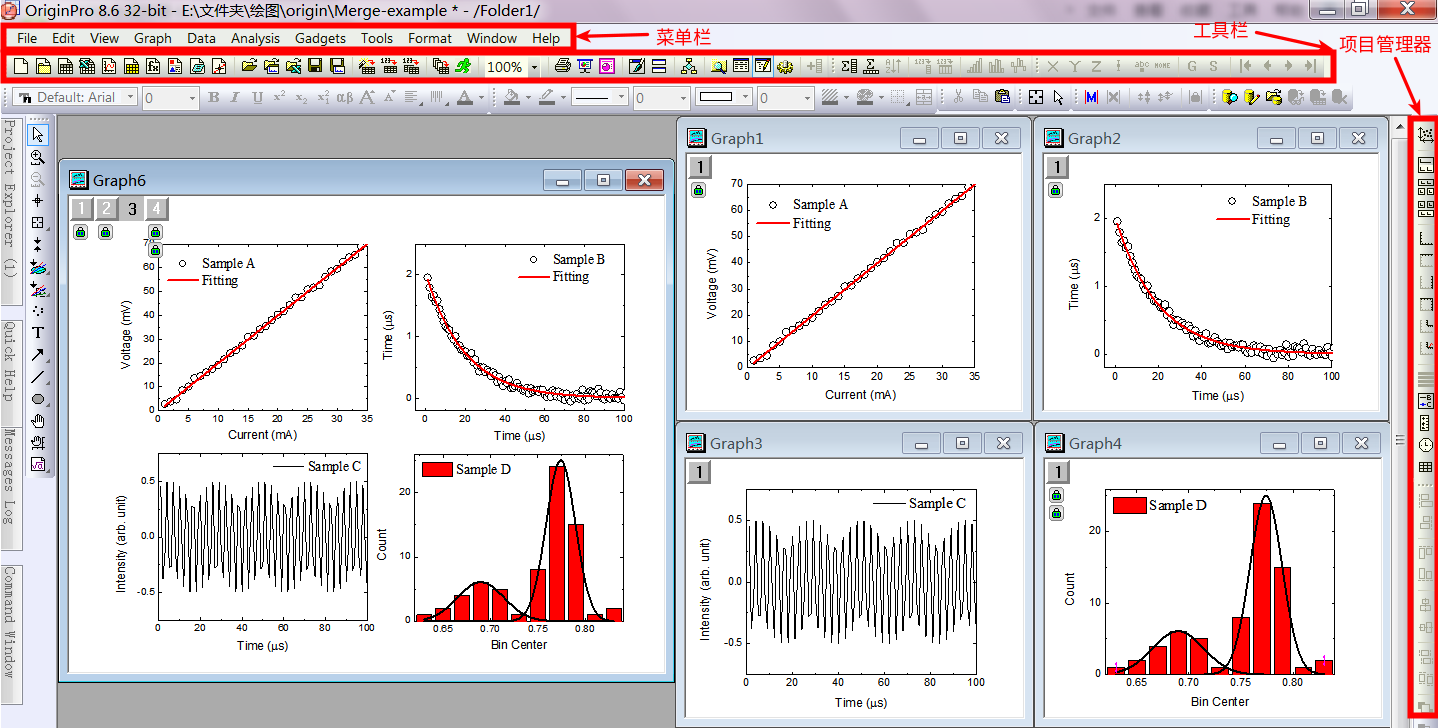
\includegraphics[height=1.75in]{Figures/Origin_Pan.png}
\label{Pan_Origin-1}
\end{figure}
}

\frame
{
	\frametitle{\textrm{Graph~}窗口简介}
	\textrm{Graph~}窗口是\textrm{Origin~}中图形处理功能最重要的组成部分。用户可在此完成制图、实现数据的可视化
	\begin{itemize}
		\item 制图包括二维图和三维图,\textcolor{magenta}{二维图是制图的基础}
	\end{itemize}
\begin{figure}[h!]
\centering
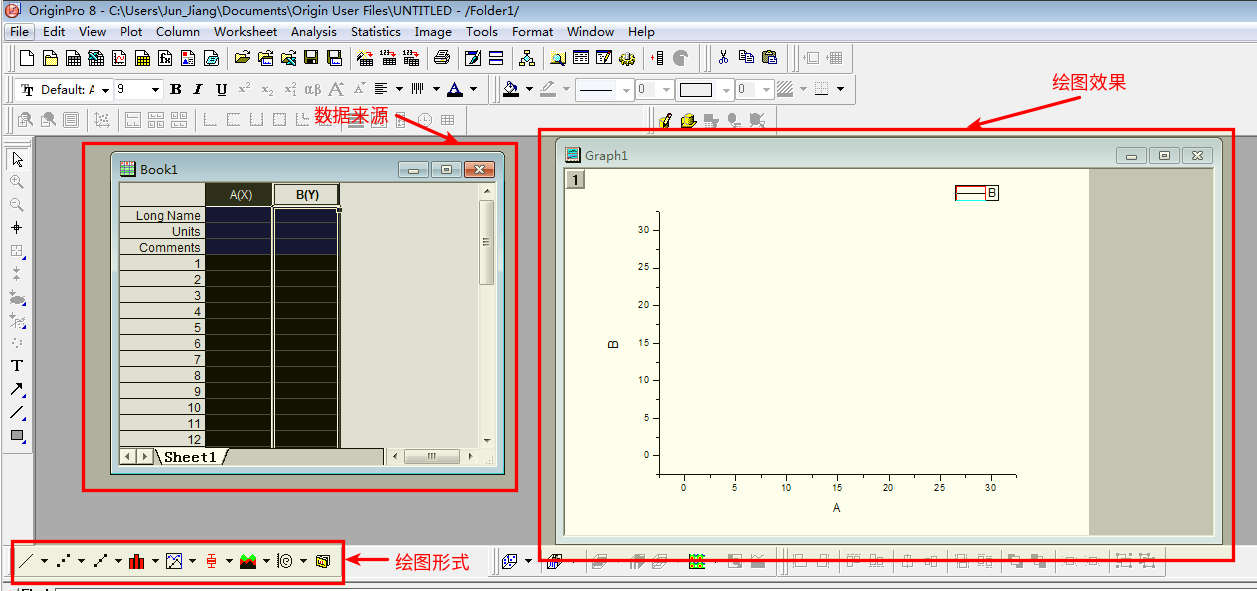
\includegraphics[height=1.85in]{Figures/Origin_Graph-2.png}
\label{Pan_Origin-2}
\end{figure}
}

\frame
{
	\frametitle{\textrm{Graph~}窗口的组成}
	\begin{itemize}
		\item \textcolor{red}{编辑页面~}编辑页面是\textrm{Graph~}制图背景,包括必要组成:~\textcolor{blue}{图层}、\textcolor{blue}{坐标轴}和\textcolor{blue}{文本}等\\
			每个编辑页面至少包含一个层
		\item \textcolor{red}{图层~}每个图层至少包含三个要素:~\textcolor{blue}{坐标轴}、\textcolor{blue}{数据制图}、\textcolor{blue}{相关文本和图标},用户可在页面内调节和移动图层的大小
		\item \textcolor{red}{框架~}绘图区的边界称为框架(\textrm{Frame})
	\end{itemize}
\begin{figure}[h!]
\centering
\vspace*{-10pt}
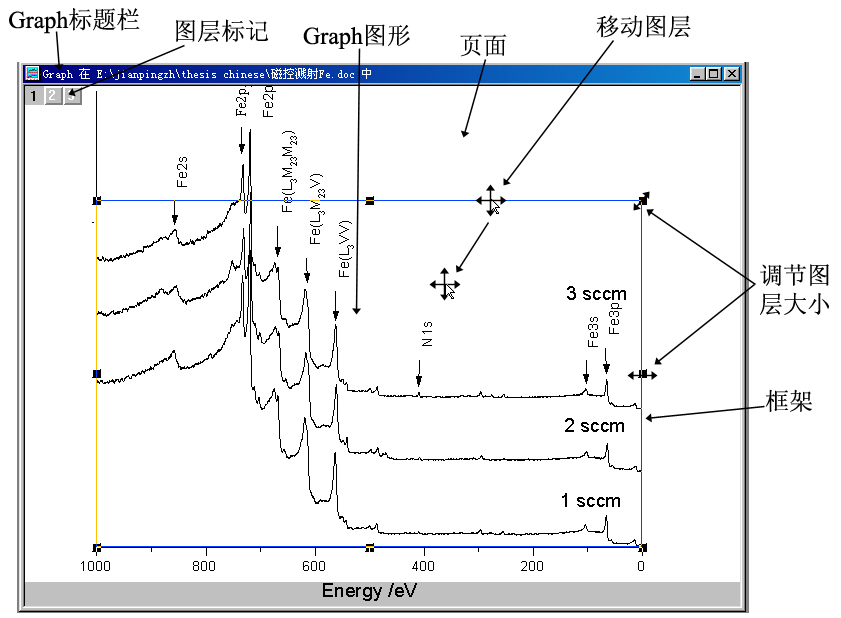
\includegraphics[height=1.65in]{Figures/Origin_Pan-2.png}
\label{Pan_Pan-2}
\end{figure}
}

\subsection{根据\rm{Worksheet}制图}
\frame
{
	\frametitle{根据\textrm{Worksheet}制图}
	选中需要绘制的\textrm{Worksheet~}数据,点击\bf{Plot|Graph~}类型,或直接单击工具条中制图模板命令按钮,获得图形
\begin{figure}[h!]
\centering
\vspace*{-5pt}
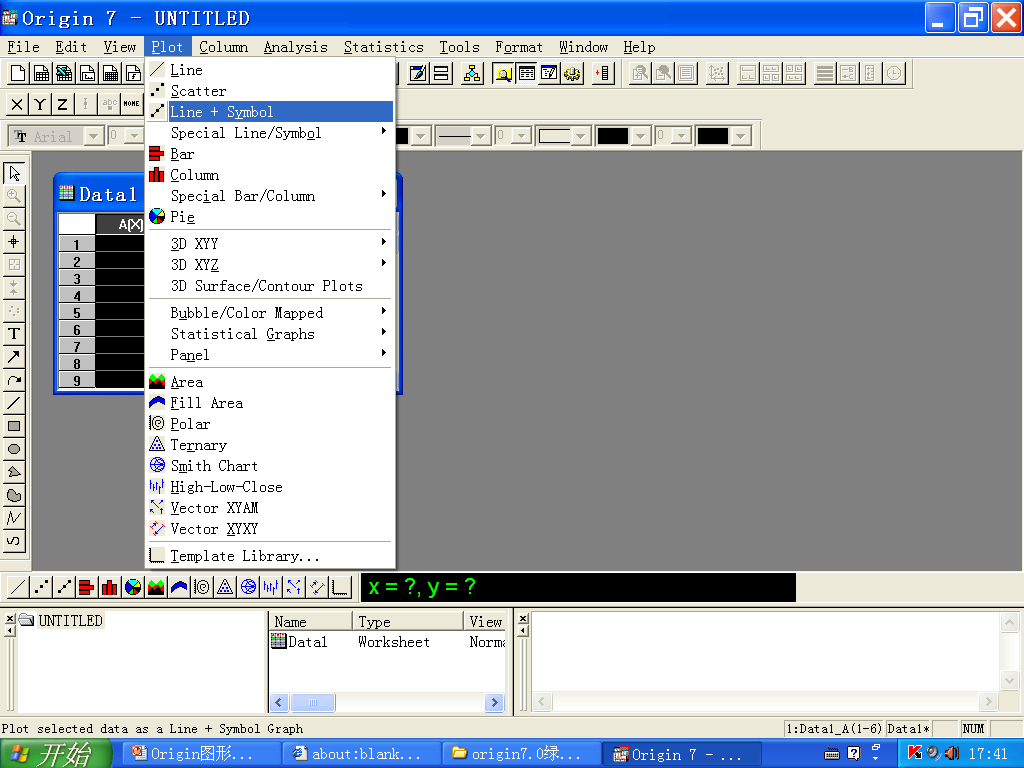
\includegraphics[height=1.55in]{Figures/Origin_Pan-3.png}
\hspace*{2pt}
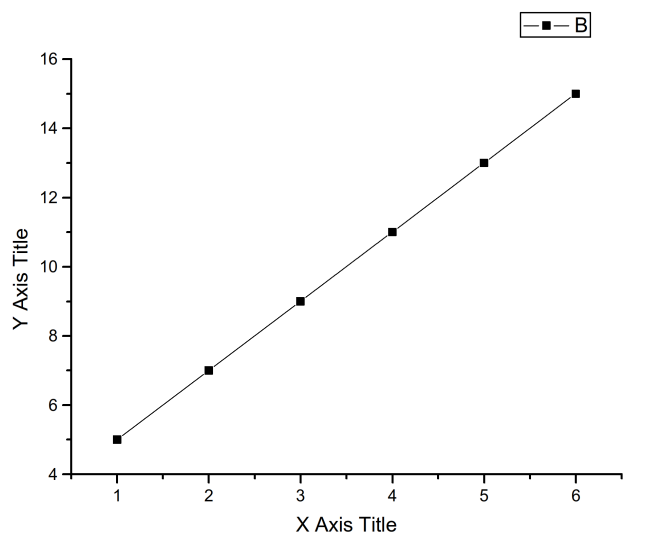
\includegraphics[height=1.55in]{Figures/Origin_Graph-3.png}
\label{Pan_Pan-3}
\end{figure}
}

\frame
{
	\frametitle{\textrm{Graph~}的模板}
	\begin{itemize}
		\item 二维\textcolor{blue}{折线}(\textrm{line})、\textcolor{blue}{散点}(\textrm{scatter})和\textcolor{blue}{折线-标号}(\textrm{line+symbol})是\textrm{Origin~}最基本的图形
		\item \textcolor{magenta}{数据要求}:~\textrm{Worksheet~}中至少有一个\bf{Y~}列,如果没有设定\bf{X}列,将行号作为\bf{X}值
	\end{itemize}
\begin{figure}[h!]
\centering
\vspace*{-10pt}
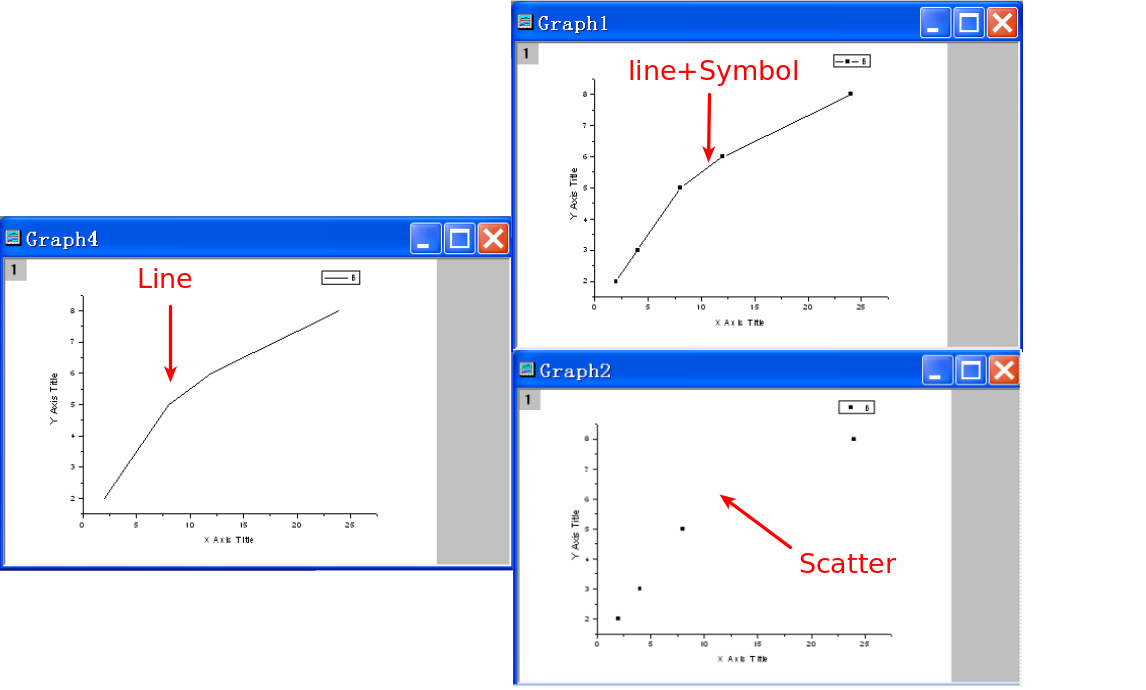
\includegraphics[height=2.05in]{Figures/Origin_Graph-4.png}
\label{Pan_Graph-4}
\end{figure}
}

\frame
{
	\frametitle{\textrm{Spline Graph~}(样条曲线)}
\begin{figure}[h!]
\centering
\vspace*{-15pt}
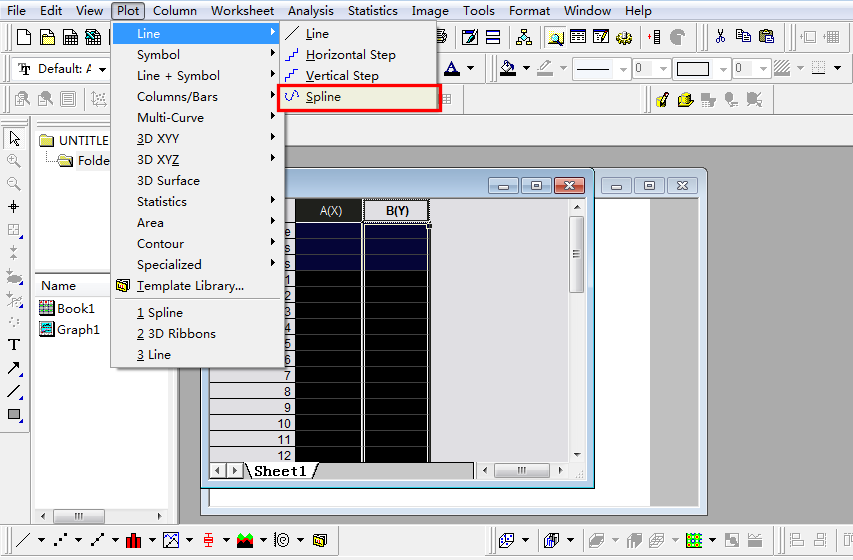
\includegraphics[height=1.35in]{Figures/Origin_Graph-5-3.png}
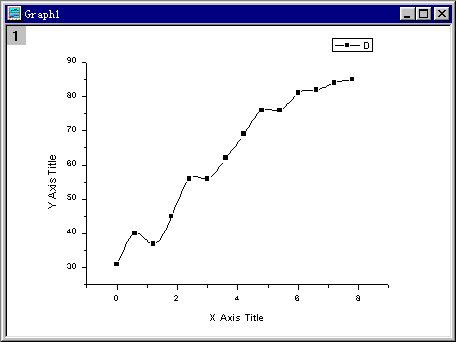
\includegraphics[height=1.35in]{Figures/Origin_Graph-5-2.png}
\vspace*{1pt}
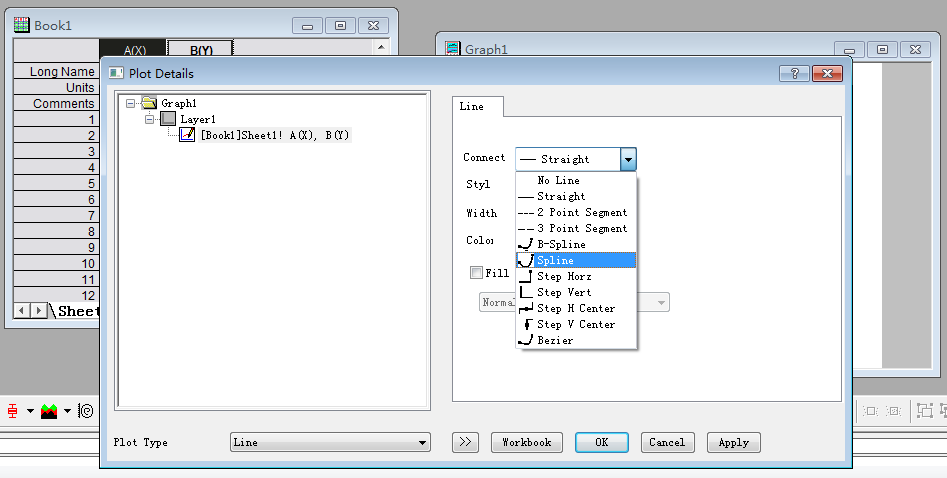
\includegraphics[height=1.65in]{Figures/Origin_Graph-5-1.png}
\label{Pan_Graph-5}
\end{figure}
}

\frame
{
	\frametitle{\textrm{Graph~}的模板}
\begin{figure}[h!]
\centering
\vspace*{-15pt}
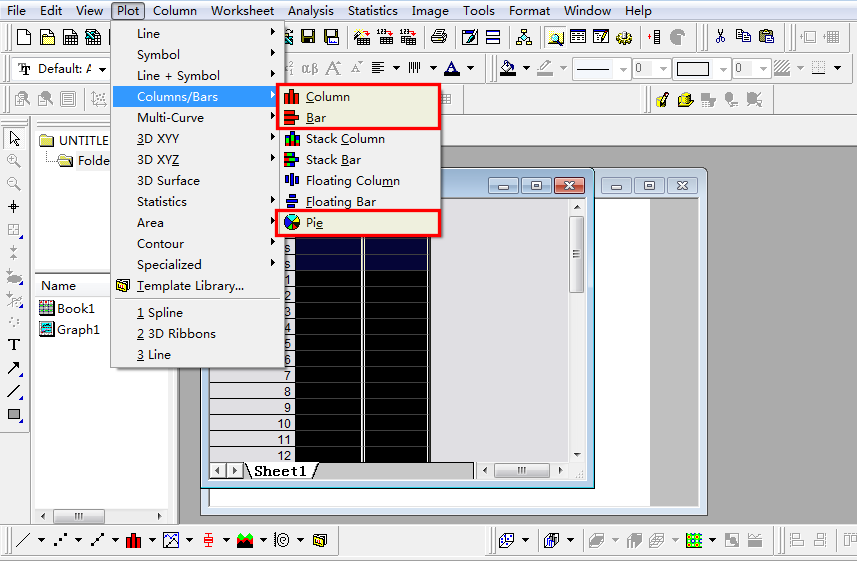
\includegraphics[height=1.40in]{Figures/Origin_Graph-6-1-1.png}
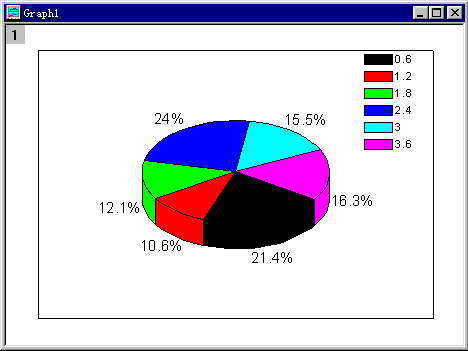
\includegraphics[height=1.40in]{Figures/Origin_Graph-6-4.png}
\vspace*{2pt}
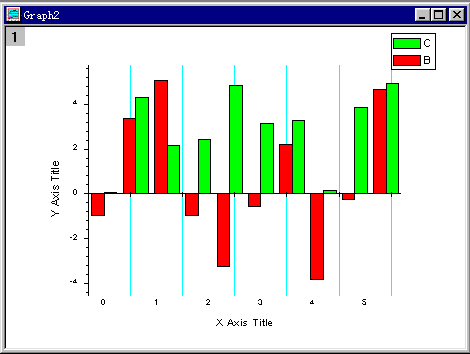
\includegraphics[height=1.50in]{Figures/Origin_Graph-6-2.png}
\hspace*{2pt}
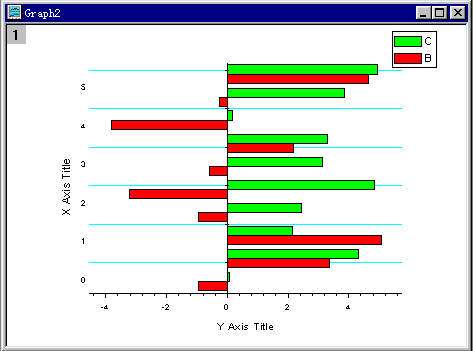
\includegraphics[height=1.50in]{Figures/Origin_Graph-6-1.png}
\label{Pan_Graph-6-1}
\end{figure}
}

\frame
{
	\frametitle{\textrm{Graph~}的模板}
\begin{figure}[h!]
\centering
\vspace*{-15pt}
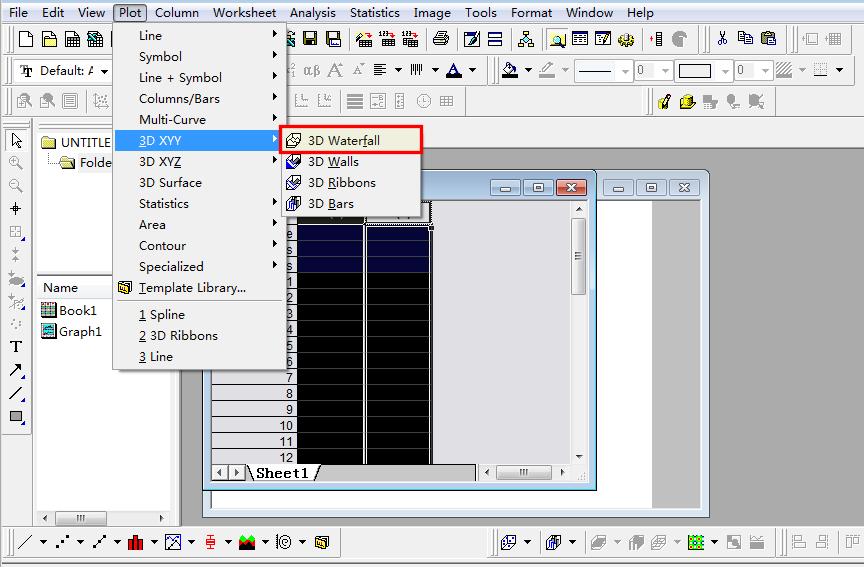
\includegraphics[height=1.50in]{Figures/Origin_Graph-6-3-1.png}
\vspace*{2pt}
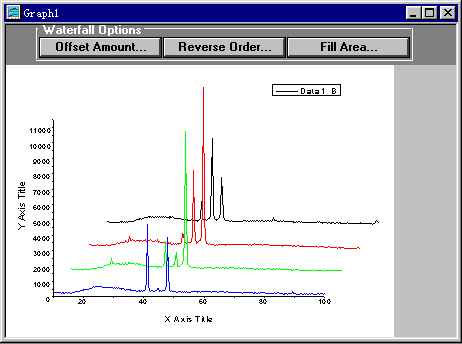
\includegraphics[height=1.50in]{Figures/Origin_Graph-6-3.png}
\label{Pan_Graph-6-3}
\end{figure}
}

\frame
{
	\frametitle{\textrm{Graph~}的模板}
\begin{figure}[h!]
\centering
\vspace*{-15pt}
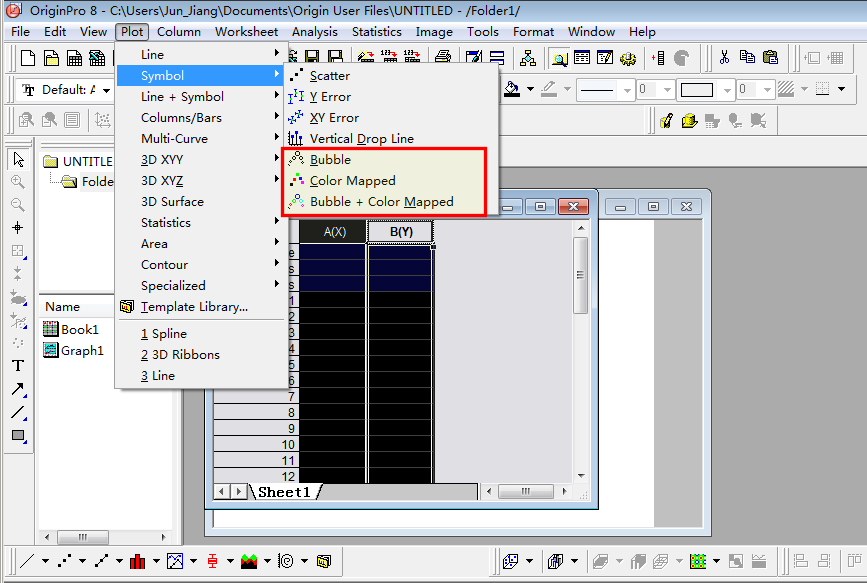
\includegraphics[height=1.50in]{Figures/Origin_Graph-6-6-1.png}
\vspace*{2pt}
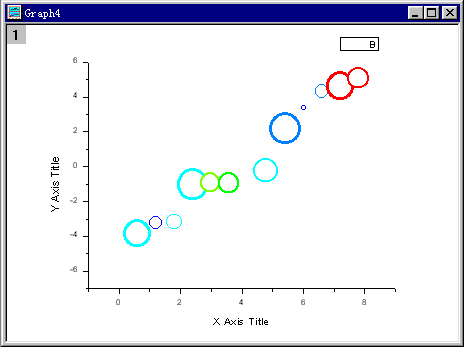
\includegraphics[height=1.50in]{Figures/Origin_Graph-6-6.png}
\hspace*{2pt}
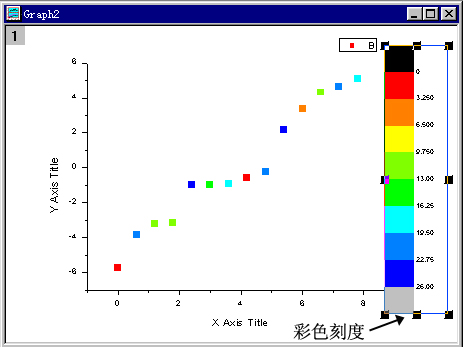
\includegraphics[height=1.50in]{Figures/Origin_Graph-6-5.png}
\label{Pan_Graph-6-6}
\end{figure}
}

\frame
{
	\frametitle{\textrm{Graph~}的数据曲线修饰}
\begin{figure}[h!]
\centering
\vspace*{-15pt}
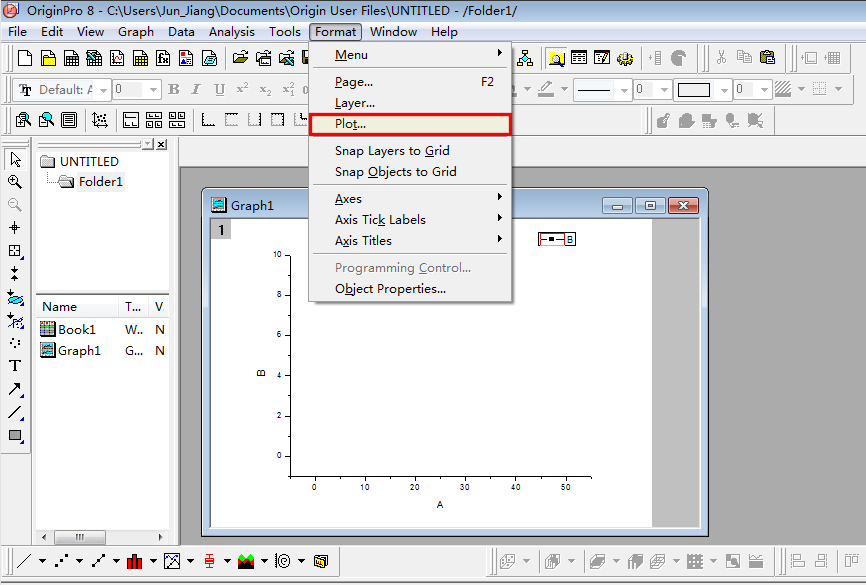
\includegraphics[height=1.50in]{Figures/Origin_Graph-7.png}
\vspace*{2pt}
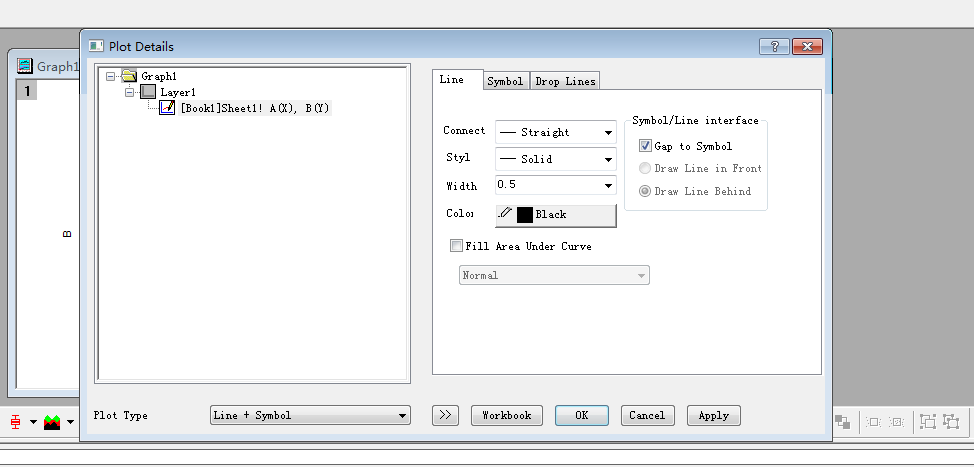
\includegraphics[height=1.40in]{Figures/Origin_Graph-7-1.png}
\hspace*{-75pt}
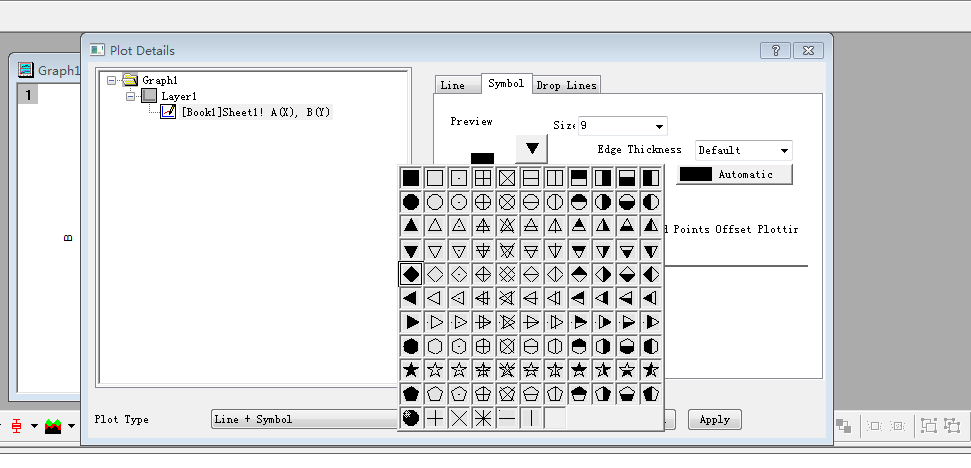
\includegraphics[height=1.40in]{Figures/Origin_Graph-7-2.png}
\label{Pan_Graph-7}
\end{figure}
}

\frame
{
	\frametitle{\textrm{Graph~}的坐标轴修饰}
\begin{figure}[h!]
\centering
\vspace*{-15pt}
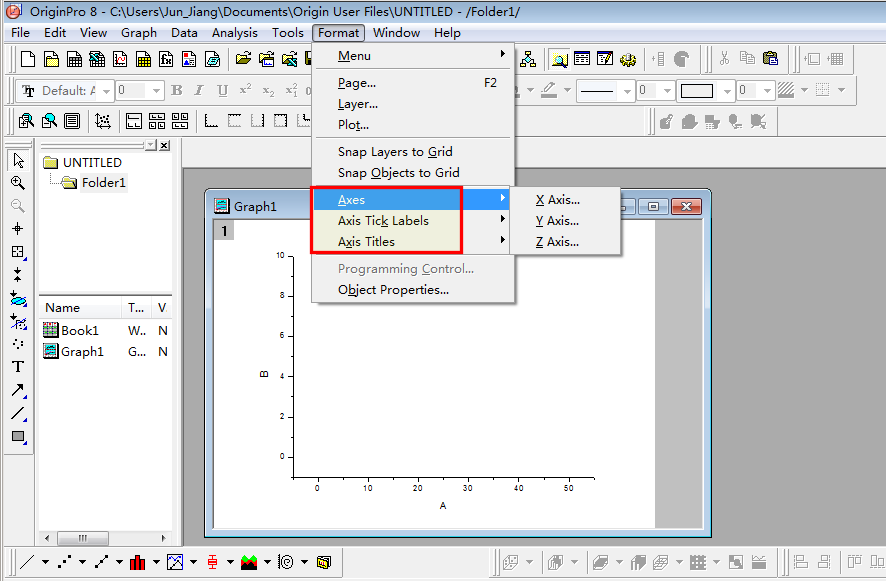
\includegraphics[height=1.40in]{Figures/Origin_Graph-8.png}
\hspace*{2pt}
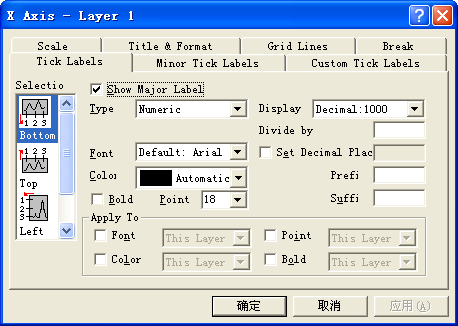
\includegraphics[height=1.40in]{Figures/Origin_Graph-8-1.png}
\vspace*{2pt}
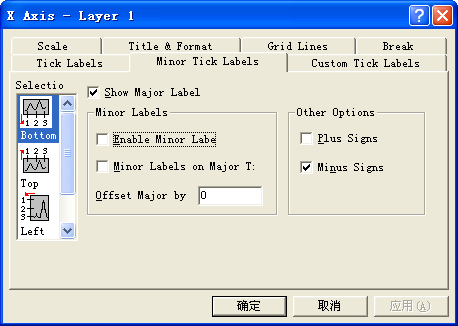
\includegraphics[height=1.40in]{Figures/Origin_Graph-8-3.png}
\hspace*{2pt}
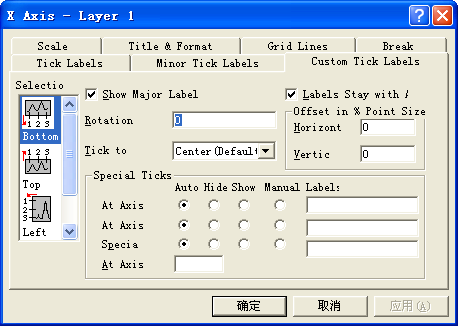
\includegraphics[height=1.40in]{Figures/Origin_Graph-8-4.png}
\label{Pan_Graph-8}
\end{figure}
}

\frame
{
	\frametitle{\textrm{Graph~}的坐标轴修饰}
\begin{figure}[h!]
\centering
\vspace*{-15pt}
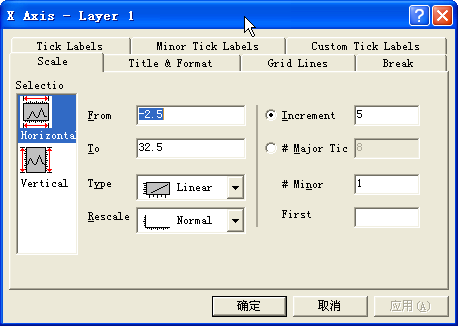
\includegraphics[height=1.40in]{Figures/Origin_Graph-8-2.png}
\hspace*{2pt}
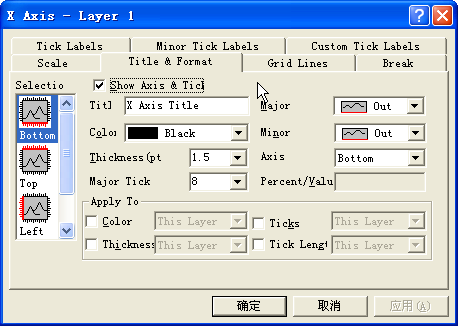
\includegraphics[height=1.40in]{Figures/Origin_Graph-8-7.png}
\vspace*{2pt}
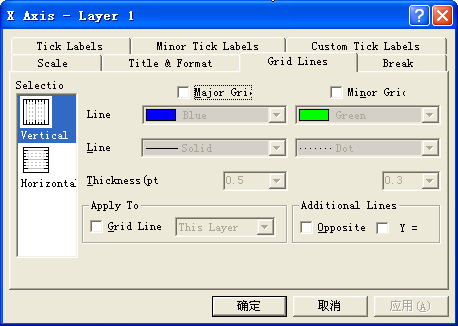
\includegraphics[height=1.40in]{Figures/Origin_Graph-8-5.png}
\hspace*{2pt}
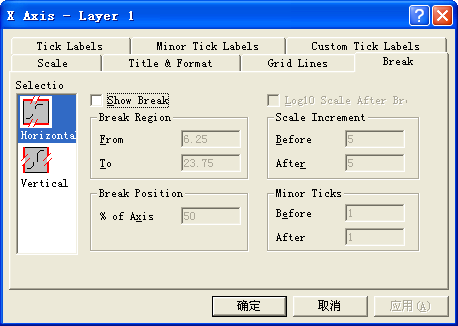
\includegraphics[height=1.40in]{Figures/Origin_Graph-8-6.png}
\label{Pan_Graph-8-2}
\end{figure}
}

\frame
{
	\frametitle{数据的导入}
\begin{figure}[h!]
\centering
\vspace*{-15pt}
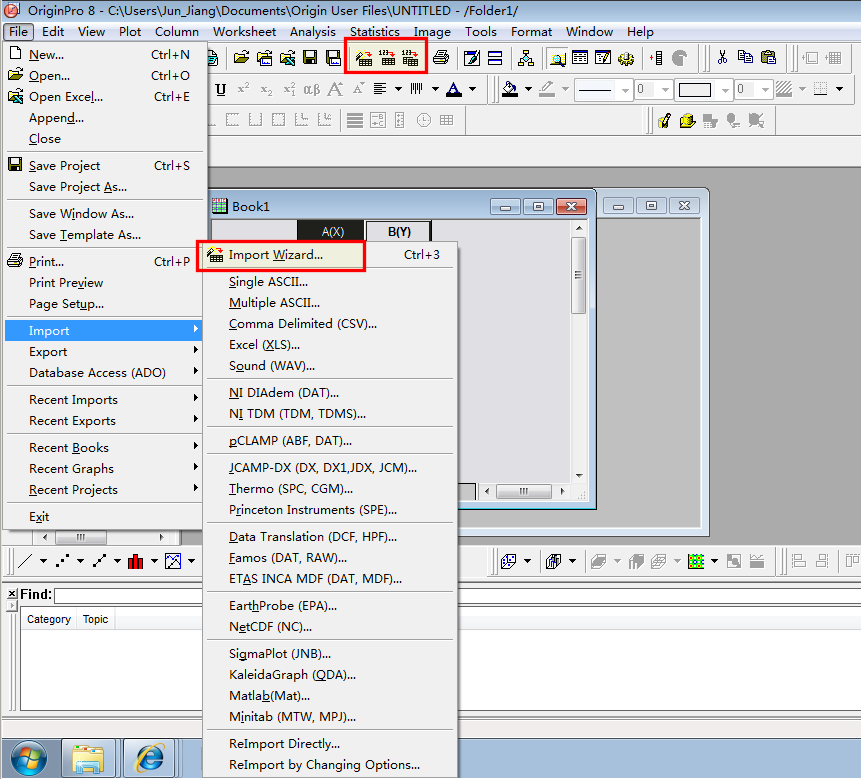
\includegraphics[height=2.70in]{Figures/Origin_Data.png}
\label{Pan_Data}
\end{figure}
}

\frame
{
	\frametitle{数据的导入}
\begin{figure}[h!]
\centering
\hspace*{-15pt}
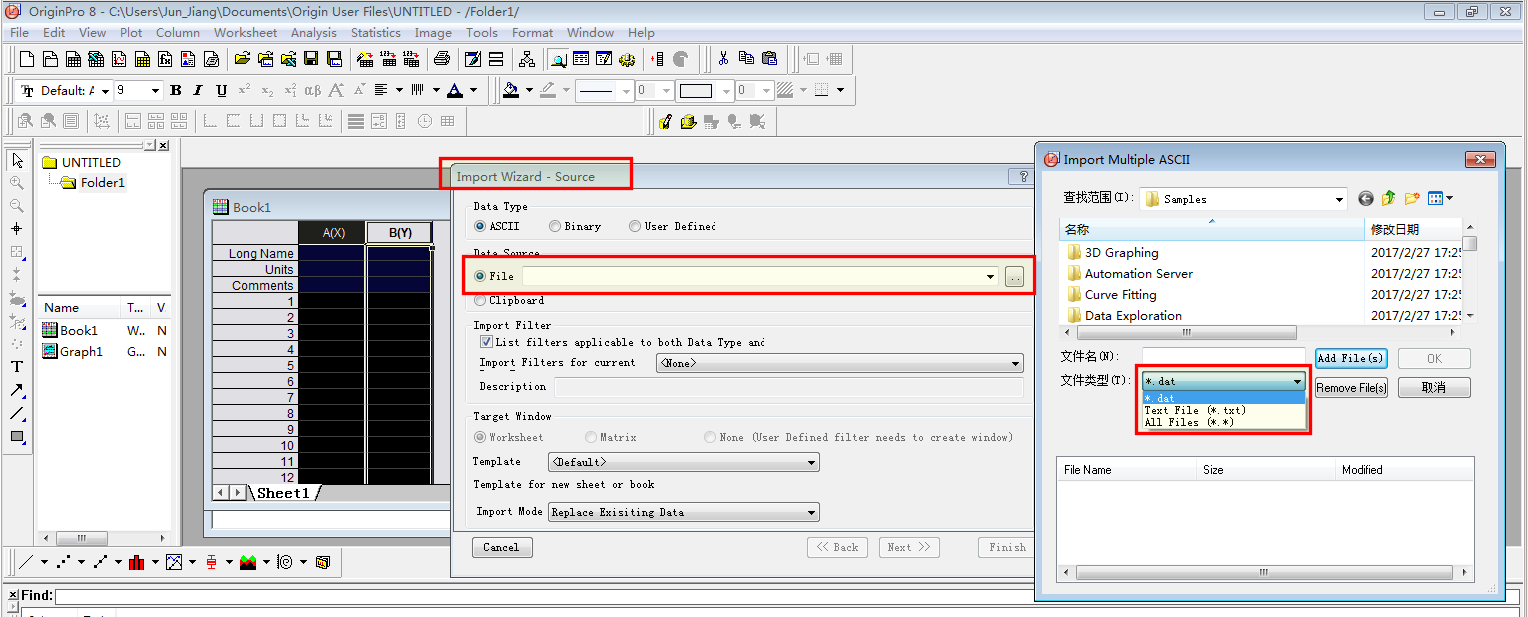
\includegraphics[height=1.80in]{Figures/Origin_Data-1.png}
\label{Pan_Data-1}
\end{figure}
}

\frame
{
	\frametitle{\textrm{Graph~}的导出}
\begin{figure}[h!]
\centering
\vspace*{-15pt}
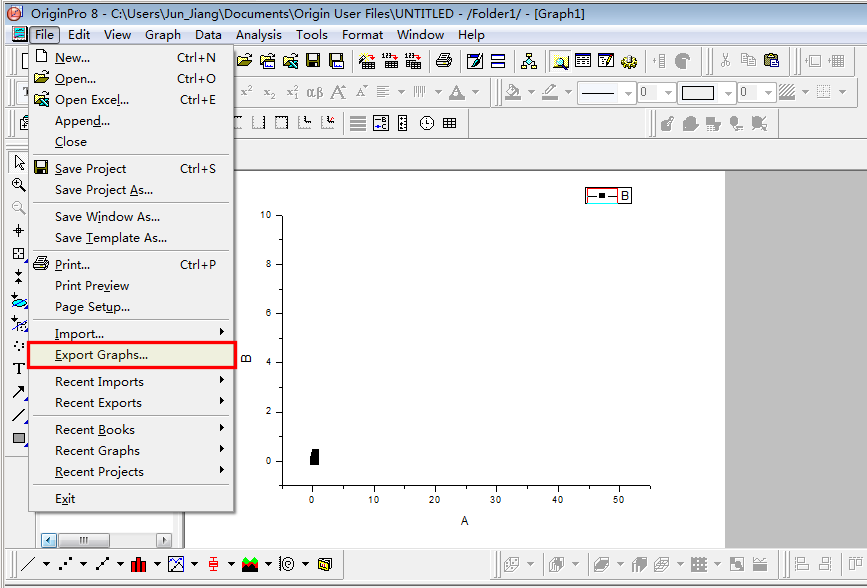
\includegraphics[height=1.50in]{Figures/Origin_Graph-9.png}
\vspace*{2pt}
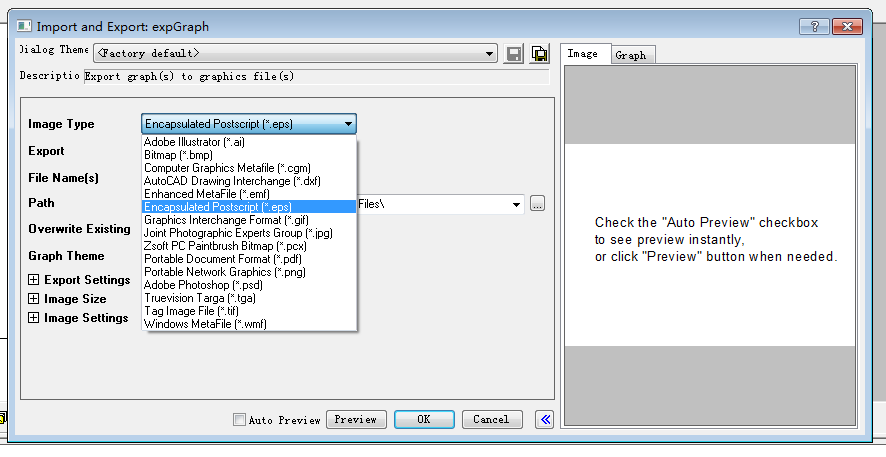
\includegraphics[height=1.40in]{Figures/Origin_Graph-9-1.png}
\hspace*{-75pt}
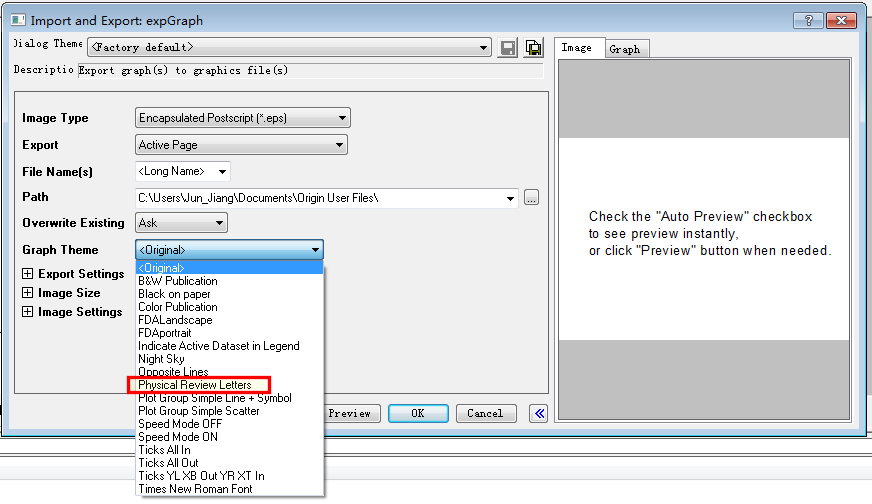
\includegraphics[height=1.40in]{Figures/Origin_Graph-9-2.png}
\label{Pan_Graph-9}
\end{figure}
}

\subsection{\rm{Origin~}的数据处理与分析}
\frame
{
	\frametitle{\textrm{Origin~}的数据处理与分析}
\begin{figure}[h!]
\centering
\vspace*{-15pt}
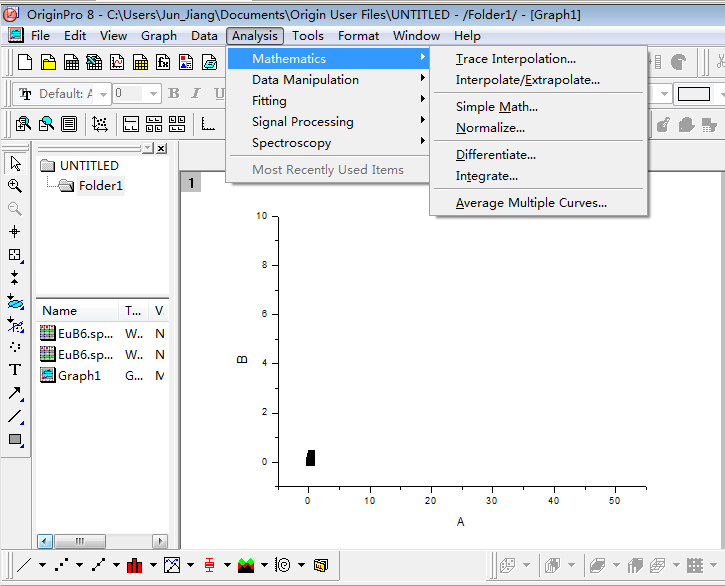
\includegraphics[height=1.50in]{Figures/Origin_Analy-2.png}
\hspace*{-5pt}
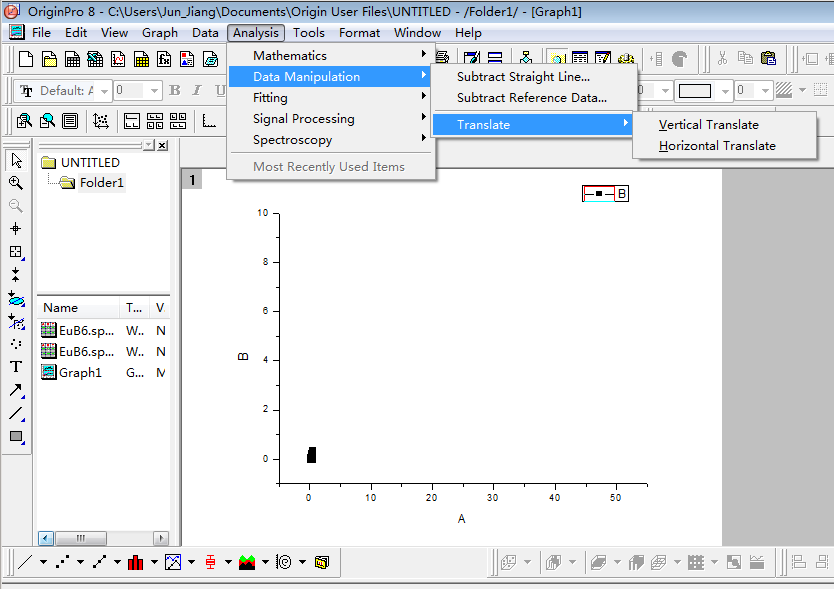
\includegraphics[height=1.50in]{Figures/Origin_Analy-3.png}
\vspace*{2pt}
\hspace*{-30pt}
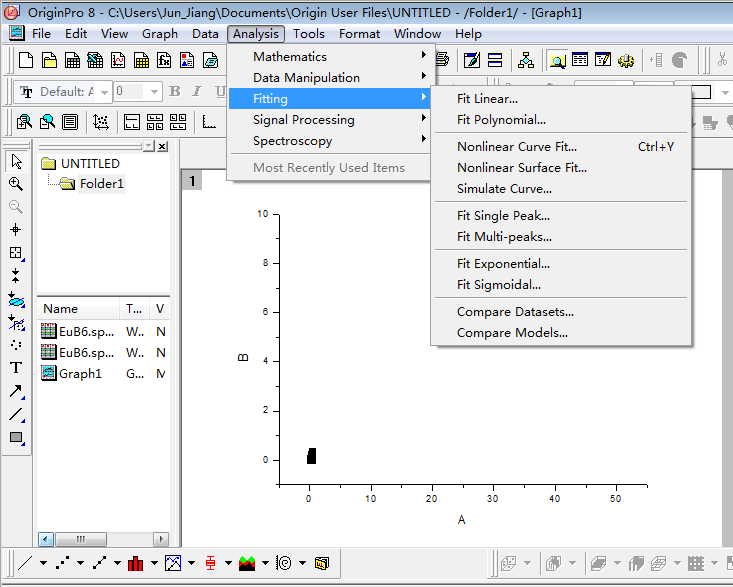
\includegraphics[height=1.50in]{Figures/Origin_Analy-1.png}
\hspace*{-25pt}
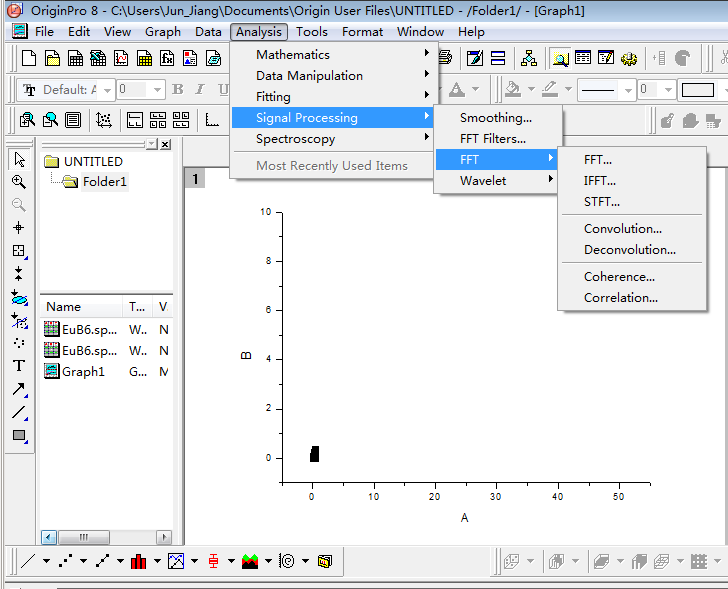
\includegraphics[height=1.50in]{Figures/Origin_Analy-4.png}
\hspace*{-15pt}
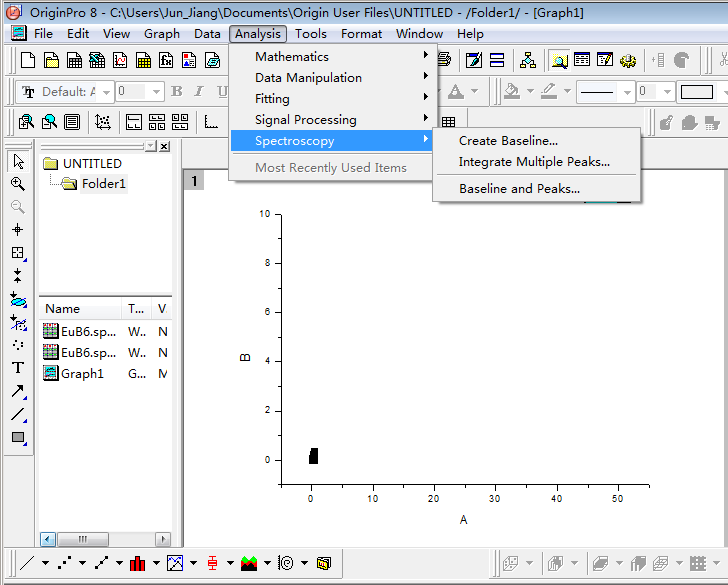
\includegraphics[height=1.50in]{Figures/Origin_Analy-5.png}
\label{Origin_Analysis}
\end{figure}
}

\frame
{
	\frametitle{\textrm{Origin~}的曲线拟合的函数}
\begin{figure}[h!]
\centering
\vspace*{-25pt}
\hspace*{-15pt}
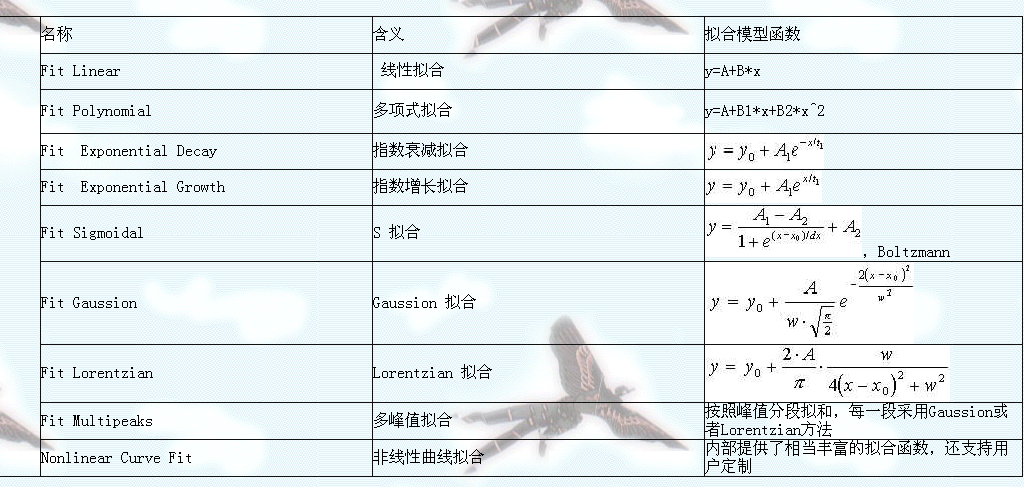
\includegraphics[height=2.1in]{Figures/Origin_Analy-fun.png}
\label{Origin_Analysis-2}
\end{figure}
}

\frame
{
	\frametitle{\textrm{Origin~}的曲线拟合举例:~线性拟合}
	\begin{itemize}
		\item \textcolor{red}{例:~}某种铝合金的含铝量为$x\%$,其熔解温度为$y^{\text{o}}\mathrm{C}$,由实验测得数据如下表所表示:~
			试用最小二乘法求一拟合曲线,使其最好地拟合这组给定的数据
\begin{figure}[h!]
\centering
\vspace*{-7pt}
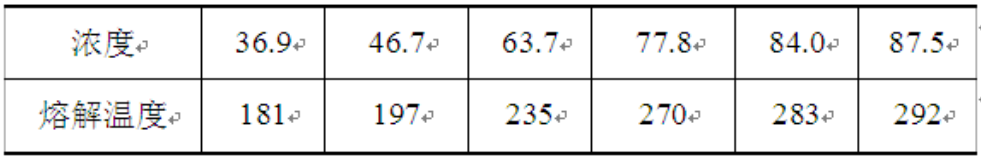
\includegraphics[height=0.6in]{Figures/Origin_example-1.png}
\label{Origin_example}
\end{figure}
	\end{itemize}
\vspace*{-10pt}
	\begin{itemize}
		\item \textcolor{red}{解:~}
			\begin{enumerate}
				\item 作草图
				\item 确定拟合曲线为直线,令
					\begin{displaymath}
						p(x)=a+bx
					\end{displaymath}
				\item 根据最小二乘法,建立方程组
					\begin{displaymath}
						\left\{
						\begin{aligned}
							&aN+b\sum x_i=\sum y_i\\
&a\sum x_i+b\sum x_i^2=\sum x_iy_i
						\end{aligned}\right.
					\end{displaymath}
			\end{enumerate}
	\end{itemize}
}

\frame
{
	\frametitle{\textrm{Origin~}的曲线拟合举例:~线性拟合}
\begin{figure}[h!]
\centering
\vspace*{-15pt}
\includegraphics[height=1.3in]{Figures/Origin_example-1-2.png}
\label{Origin_example-1-1}
\end{figure}
由上表可得
\begin{displaymath}
	\left\{
	\begin{aligned}
		&6a+396.9b=1458\\
&396.9a+28365.28b=101176.3
	\end{aligned}\right.
\end{displaymath}
解得方程:~
\begin{displaymath}
	\left\{
		\begin{aligned}
			&a=95.3524\\
			&b=2.2337
		\end{aligned}
		\right.
\end{displaymath}
即经验公式为
\begin{displaymath}
	p(x)=95.3524+2.2337x
\end{displaymath}
}

\frame
{
	\frametitle{\textrm{Origin~}的曲线拟合举例:~线性拟合}
\begin{figure}[h!]
\centering
\vspace*{-15pt}
\includegraphics[height=2.7in]{Figures/Origin_example-1-3.png}
\label{Origin_example-1-3}
\end{figure}
}

\frame
{
	\frametitle{\textrm{Origin~}的曲线拟合举例:~多项式拟合}
	\begin{itemize}
		\item \textcolor{red}{例:~}设在某一实验中观测两个变量$x$和$y$,得到一组数据如下表所示。求一代数多项式,使其最好得拟合这组给定的数据。
\begin{figure}[h!]
\centering
\vspace*{-10pt}
\includegraphics[height=0.6in]{Figures/Origin_example-2.png}
\label{Origin_example-2}
\end{figure}
	\end{itemize}
	\begin{itemize}
		\item \textcolor{red}{解:~}
			\begin{enumerate}
				\item 作草图
				\item 确定拟合曲线的形式,由图中可知,可用抛物线拟合该组实验数据,令
					\begin{displaymath}
						y=a+bx+cx^2
					\end{displaymath}
			\end{enumerate}
	\end{itemize}
}

\frame
{
	\frametitle{\textrm{Origin~}的曲线拟合举例:~多项式拟合}
	类似地,根据最小二乘法,可有
\begin{figure}[h!]
\centering
\vspace*{-5pt}
\includegraphics[height=0.9in]{Figures/Origin_example-2-1.png}
\label{Origin_example-2-1}
\end{figure}
由表中可得
\begin{displaymath}
	\left[
		\begin{matrix}
			9 & 53 & 381\\
			53 &381 &3017\\
			381 &3017 &25317
		\end{matrix}
		\right]\left[
			\begin{matrix}
				a \\ b\\ c
			\end{matrix}
			\right]=\left[
				\begin{matrix}
					32 \\ 147 \\ 1025
				\end{matrix}
				\right]
\end{displaymath}
解此方程可得:
\begin{displaymath}
	a=13.4597,\quad b=-3.6053,\quad c=0.2676
\end{displaymath}
所求得的拟合多项式为:~
\begin{displaymath}
	y=13.4597-3.6053x+0.2676x^2
\end{displaymath}
}


\frame
{
	\frametitle{\textrm{Origin~}的曲线拟合举例:~多项式拟合}
\begin{figure}[h!]
\centering
\vspace*{-15pt}
\includegraphics[height=2.7in]{Figures/Origin_example-2-2.png}
\label{Origin_example-2-2}
\end{figure}
}

\frame
{
	\frametitle{\textrm{Origin~}的曲线拟合举例:~插值}
	\begin{itemize}
		\item \textcolor{red}{例:~}利用开方关系
			\begin{displaymath}
				\sqrt{100}=10,\quad\sqrt{121}=11,\quad\sqrt{144}=12
			\end{displaymath}
			求$\sqrt{115}$的值
		\item \textcolor{red}{解:~}利用上述抛物线插值,
			\begin{displaymath}
				\begin{aligned}
					&x_0=100,\quad\quad y_0=10 \\
&x_1=121,\quad\quad y_1=11 \\
&x_2=144,\quad\quad y_2=12
				\end{aligned}
			\end{displaymath}
			可以解得:
			\begin{displaymath}
				\sqrt{115}=10.7228
			\end{displaymath}
	\end{itemize}
}

\frame
{
	\frametitle{\textrm{Origin~}的曲线拟合举例:~插值}
\begin{figure}[h!]
\centering
\vspace*{-5pt}
\includegraphics[height=2.30in]{Figures/Origin_example-3-1.png}
\hspace*{-15pt}
\includegraphics[height=2.30in]{Figures/Origin_example-3-2.png}
\label{Origin_example-3}
\end{figure}
}

\frame
{
	\frametitle{\textrm{Origin~}的曲线拟合举例:~插值}
\begin{figure}[h!]
\centering
\vspace*{-5pt}
\includegraphics[height=2.20in]{Figures/Origin_example-3-3.png}
\hspace*{-28pt}
\includegraphics[height=1.75in]{Figures/Origin_example-3.png}
\label{Origin_example-3-2}
\end{figure}
}

\section{\rm{MATLAB~}绘图的基础}
\frame
{
	\frametitle{\textrm{Matlab~}的图形窗口}
	\begin{itemize}
		\item 创建图形窗口命令\textcolor{red}{\bf{figure}}\\
			调用格式: \textcolor{blue}{\textrm{figure}}/\textcolor{blue}{\textrm{figure(n)}}\\
		\textcolor{red}{例:~}
\begin{figure}[h!]
\centering
\vspace*{-15pt}
\includegraphics[height=1.60in]{Figures/Matlab_figure-1.png}
\label{Matlab_figure}
\end{figure}
		\item 由菜单创建图形窗口:\\
			\textcolor{magenta}{\bf{File}}$\Rightarrow$\textcolor{magenta}{\bf{New}}$\Rightarrow$\textcolor{magenta}{\bf{Figure}}
	\end{itemize}
}

\subsection{简易绘图函数}
\frame
{
	\frametitle{符号数学的简易绘图函数}
	\begin{itemize}
		\item 二维简易绘图函数
			\begin{enumerate}
				\item \textcolor{red}{\bf ezplot}($f$):~绘制表达式$f(x)$的二维图形
				\item \textcolor{red}{\bf ezplot}($f$,$[x_{\mathrm{min}},x_{\mathrm{max}}]$):~绘制表达式$f(x)$的二维图形,指定$x$的取值范围$[x_{\mathrm{min}},x_{\mathrm{max}}]$
			\end{enumerate}
		\item \textcolor{red}{优点:~}命令使用极简单,只需指定绘图函数名
		\item \textcolor{red}{缺点:~}功能简单,主要适用于绘制显式函数图形
	\end{itemize}
		\textcolor{red}{例:~}绘制表达式$x^2-y^4$的二维图形
\begin{figure}[h!]
\centering
\vspace*{-5pt}
\includegraphics[height=1.30in]{Figures/Matlab_ezplot-1.png}
\label{Matlab_ezplot-1}
\end{figure}
}

\frame
{
	\frametitle{符号数学的简易绘图函数}
	二维绘图函数\\
	\textcolor{red}{例:~}绘制误差函数$\mathrm{erf}(x)=\dfrac2{\sqrt{\pi}}\int_0^x\mathrm{e}^{-t^2}\mathrm{d}t$
\begin{figure}[h!]
\centering
\vspace*{-5pt}
\includegraphics[height=2.00in]{Figures/Matlab_ezplot-2.png}
\label{Matlab_ezplot-2}
\end{figure}
}

\frame
{
	\frametitle{符号数学的简易绘图函数}
	三维绘图函数
	\begin{enumerate}
		\item \textcolor{red}{\bf ezplot3}:~绘制$x=x(t)$,$y=y(t)$,$z=z(t)$定义的三维图形
		\item \textcolor{red}{\bf ezplot3}($x$,$y$,$z$,$[t_{\mathrm{min}},t_{\mathrm{max}}]$):~指定绘图范围$[t_{\mathrm{min}},t_{\mathrm{max}}]$
		\item \textcolor{red}{\bf ezplot3}($x$,$y$,$z$,$[t_{\mathrm{min}},t_{\mathrm{max}}]$,'\textcolor{blue}{animate}'):~绘制三维动态轨迹图
	\end{enumerate}
	\textcolor{red}{例:~}根据$x=\sin(t)$,$y=\cos(t)$,$z=t$绘制三维曲线
\begin{figure}[h!]
\centering
\vspace*{-5pt}
\includegraphics[height=1.70in]{Figures/Matlab_ezplot3-1.png}
\label{Matlab_ezplot3-1}
\end{figure}
}

\frame
{
	\frametitle{符号数学的简易绘图函数}
	等高线绘图函数
	\begin{enumerate}
		\item \textcolor{red}{\bf ezcontour}($f$):~绘制函数$f=f(x,y)$定义的等高线
		\item \textcolor{red}{\bf ezcontour}($f$,\textcolor{green}{domain}):~绘制函数$f=f(x,y)$定义的等高线,\textcolor{green}{domain}定义自变量$x$和$y$的取值范围
	\end{enumerate}
	\textcolor{red}{例:~}根据表达式绘制$f$的等高线
	\begin{displaymath}
		f=3(1-x)^2\mathrm{e}^{-x^2-(1+y)^2}-10(\frac{x}5-x^3-y^2)\mathrm{e}^{-x^2-y^2}-\frac13\mathrm{e}^{-(x+1)^2-y^2}
	\end{displaymath}
\begin{figure}[h!]
\centering
\vspace*{-10pt}
\includegraphics[height=1.50in]{Figures/Matlab_ezcontour-1.png}
\label{Matlab_ezcontour-1}
\end{figure}
}

\frame
{
	\frametitle{符号数学的简易绘图函数}
	等高线绘图填充函数~\textcolor{red}{\bf ezcontour\underline{f}}\\
	\textcolor{red}{例:~}根据表达式绘制$f$的\textcolor{cyan}{填充}等高线
	\begin{displaymath}
		f=3(1-x)^2\mathrm{e}^{-x^2-(1+y)^2}-10(\frac{x}5-x^3-y^2)\mathrm{e}^{-x^2-y^2}-\frac13\mathrm{e}^{-(x+1)^2-y^2}
	\end{displaymath}
\begin{figure}[h!]
\centering
\vspace*{-15pt}
\includegraphics[height=1.90in]{Figures/Matlab_ezcontour-2.png}
\label{Matlab_ezcontour-2}
\end{figure}
}

\frame
{
	\frametitle{符号数学的简易绘图函数}
	网格图绘图函数~\textcolor{red}{\bf ezmesh}\\
	\textcolor{red}{例:~}绘制函数$f=x\mathrm{e}^{-x^2-y^2}$的网格图
\begin{figure}[h!]
\centering
\vspace*{-5pt}
\includegraphics[height=2.20in]{Figures/Matlab_ezmesh-1.png}
\label{Matlab_ezmesh-1}
\end{figure}
}

\frame
{
	\frametitle{符号数学的简易绘图函数}
	表面图绘图函数~\textcolor{red}{\bf ezsurf}\\
	\textcolor{red}{例:~}绘制以下函数的的表面图
	\begin{displaymath}
		\begin{aligned}
			&x=\cos(s)\cos(t) \\
			&y=\cos(s)\sin(t) \\
			&z=\sin(s)
		\end{aligned}
	\end{displaymath}
\begin{figure}[h!]
\centering
\vspace*{-10pt}
\includegraphics[height=1.80in]{Figures/Matlab_ezsurf-1.png}
\label{Matlab_ezsurf-1}
\end{figure}
}

\subsection{二维和三维图形绘制与修饰、控制}
\frame
{
	\frametitle{\textrm{Matlab~}的绘图基本命令}
	\begin{itemize}
		\item 绘图的基本命令
			\begin{enumerate}
				\item 线性坐标曲线绘图命令\;\textcolor{red}{\bf{plot}}
				\item 离散曲线绘图命令\;\textcolor{red}{\bf{stem}}
			\end{enumerate}
	\end{itemize}
	函数命令\textcolor{red}{\bf{plot}}是\textrm{MATLAB~}二维曲线绘图中最简单、最重要、使用最广泛的线性绘图函数。可以生成\textcolor{blue}{线段}、\textcolor{blue}{曲线}和\textcolor{blue}{参数方程曲线}的函数图形
	\begin{itemize}
		\item \textcolor{red}{\bf{plot}}命令格式
			\begin{itemize}
				\item \textcolor{blue}{\textrm{plot(y)}}:~单参数式(\textrm{y}是纵坐标向量,横坐标向量$[1,2,3,4,\cdots]$)
				\item \textcolor{blue}{\textrm{plot(x,y)}}:~参数式(\textrm{x}是横坐标向量,\textrm{y}是纵坐标向量)
				\item \textcolor{blue}{\textrm{plot({\bf Y})}}:~$m\times n$~矩阵式(矩阵的每列为纵坐标,横坐标为向量$[1:m]$)
				\item \textcolor{blue}{\textrm{plot}({\bf X},{\bf Y})}:~混合式
				\item \textcolor{blue}{\textrm{plot({\bf Z})}}:~复向量式
				\item \textcolor{blue}{\textrm{plot(x$_1$,y$_1$,x$_2$,y$_2$,$\cdots$)}}:~综合调用方式
			\end{itemize}
	\end{itemize}
}


\frame
{
	\frametitle{\textrm{Matlab~}的绘图基本命令}
	在\textcolor{orange}{混合式}命令格式\textcolor{blue}{\textrm{plot}({\bf X},{\bf Y})}中,{\bf X}和{\bf Y}可分为如下情形:
	\begin{itemize}
		\item 如果{\bf X}和{\bf Y}都是向量,\textcolor{red}{要求长度相等}
		\item 如果{\bf X}是向量,{\bf Y}是矩阵,{\bf X}的长度与{\bf Y}的行数或列数相等,则将矩阵{\bf Y}的每列或每行的向量对应{\bf X}作折(曲)线;当{\bf Y}是\textcolor{red}{方阵}时,向量{\bf X}与矩阵{\bf Y}的\textcolor{red}{列向量}对应作图
		\item 如果{\bf X}是矩阵,{\bf Y}是向量,{\bf Y}的长度与{\bf X}的行数或列数相等,则将矩阵{\bf X}的每列或每行的向量对应{\bf Y}作折图;当{\bf X}是\textcolor{red}{方阵}时,矩阵{\bf X}的\textcolor{red}{各列向量}与{\bf Y}对应作图
		\item 如果{\bf X}与{\bf Y}都是矩阵,且维度相同,则按\textcolor{red}{列对列}的方式来作图
	\end{itemize}
				\textcolor{blue}{\textrm{plot(x,y,'\textcolor{cyan}{s}')}}:~开关格式,字符串\textcolor{cyan}{s}设定图形曲线的颜色、线型和标记符号
}

\frame
{
	\frametitle{图形颜色、标记和线性参数表}
\begin{figure}[h!]
\centering
\vspace*{-10pt}
\hspace*{-65pt}
\includegraphics[height=2.10in]{Figures/Matlab_plot_s.png}
\label{Matlab_plot_s}
\end{figure}
}

\frame
{
	\frametitle{简单作图举例}
\begin{figure}[h!]
\centering
\hspace*{-15pt}
\includegraphics[height=1.85in]{Figures/Matlab_plot-1.png}
\hspace{2pt}
\includegraphics[height=1.85in]{Figures/Matlab_plot-2.png}
\label{Matlab_plot_1}
\end{figure}
}

\frame
{
	\frametitle{简单作图举例}
\begin{figure}[h!]
\centering
\vspace*{-15pt}
\includegraphics[height=2.05in]{Figures/Matlab_plot-3.png}
\label{Matlab_plot_3}
\end{figure}

\begin{itemize}
	\item 曲线1:~红色实线,$+$号表示数据点
	\item 曲线2:~黑色虚线(点线),$*$号表示数据点
	\item 曲线3:~蓝色双划虚线,$\triangle$表示数据点
\end{itemize}
}

\frame
{
	\frametitle{简单作图举例}
\begin{figure}[h!]
\centering
\hspace*{-65pt}
\vspace*{-45pt}
\includegraphics[height=2.85in]{Figures/Matlab_plot-load.png}
\label{Matlab_plot_load}
\end{figure}
}

\frame
{
	\frametitle{图形的修饰与控制}
\begin{enumerate}
	\item \textcolor{orange}{\bf title}:~图形标题
	\item \textcolor{orange}{\bf xlable/ylabel}:~$x/y$轴标注
	\item \textcolor{orange}{\bf text}:~图形任意指定位置标注
	\item \textcolor{orange}{\bf gtext}:~用鼠标将标注加到指定位置
	\item \textcolor{orange}{\bf grid on/off~grid}:~网络线开关
	\item \textcolor{orange}{\bf legend}:~标注图例
	\item \textcolor{orange}{\bf axis}:~控制坐标刻度
	\item \textcolor{orange}{\bf hold on/off~hold}:~图形叠加/撤销
	\item \textcolor{orange}{\bf subplot}:~显示多窗口子图
	\item \textcolor{orange}{\bf figure}:~多窗口绘图
\end{enumerate}
}

\frame
{
	\frametitle{图形修饰举例}
\begin{figure}[h!]
\centering
%\vspace*{-05pt}
\includegraphics[height=2.35in]{Figures/Matlab_plot-4.png}
\label{Matlab_plot_4}
\end{figure}
}

\frame
{
	\frametitle{图形修饰举例}
\begin{figure}[h!]
\centering
%\vspace*{-05pt}
\includegraphics[height=2.35in]{Figures/Matlab_plot-5.png}
\label{Matlab_plot_5}
\end{figure}
}

\frame
{
	\frametitle{图形的修饰与控制}
	在图形窗口中绘制子图形:~\textcolor{red}{\bf subplot}($m$,$n$,$p$)\\
	\begin{itemize}
		\item 图形分成$m\times n$个子窗口,并把窗口$p$指定为当前窗口
		\item 子窗口的排序:~\textcolor{violet}{从左往右~从上到下}
	\end{itemize}
\begin{figure}[h!]
\centering
\vspace*{-10pt}
\includegraphics[height=2.15in]{Figures/Matlab_plot-6.png}
\label{Matlab_plot_6}
\end{figure}
}

\frame
{
	\frametitle{图形的修饰与控制}
	多个图形窗口绘制图形:~\textcolor{red}{\bf figure}($n$)\\
	\begin{itemize}
		\item 多窗口绘图时,需按序号创建窗口,并在指定窗口中绘图
	\end{itemize}
\begin{figure}[h!]
\centering
\vspace*{-10pt}
\includegraphics[height=2.15in]{Figures/Matlab_plot-7.png}
\label{Matlab_plot_7}
\end{figure}
}

\frame
{
	\frametitle{图形的修饰与控制}
	对比绘图显示,根据需要调整绘图刻度:~\textcolor{red}{\bf hold}\\
	\begin{itemize}
		\item \textcolor{red}{\bf hold on}~保留当前图形和坐标全部属性,后续绘制的图形附加于此
		\item \textcolor{red}{\bf hold off}~缺省模式,后续作图将抹去当前图形,并重新设置坐标属性
		\item \textcolor{red}{\bf hold}~切换\textcolor{red}{\bf hold on}与\textcolor{red}{\bf hold off}两种状态

	\end{itemize}
\begin{figure}[h!]
\centering
\vspace*{-10pt}
\includegraphics[height=1.65in]{Figures/Matlab_plot-8.png}
\label{Matlab_plot_8}
\end{figure}
}

\frame
{
	\frametitle{二维函数曲线专用命令}
	\begin{itemize}
		\item 用\textcolor{red}{\bf plot}绘图,自变量一般采用\textcolor{magenta}{平均间隔}
		\item \textcolor{red}{\bf fplot}是绘制函数$y=f(x)$图形专用命令,\textcolor{magenta}{数据点自适应产生},用\textcolor{red}{\bf fplot}绘图更接近真实\\
			\textcolor{red}{\bf fplot}的调用格式:~\\
			\textcolor{blue}{[X,Y]=fplot(fun,lims,tol,n,'linespec',p$_1$,p$_2$,$\cdots$)}
	\begin{itemize}
		\item \textcolor{blue}{fun}:~函数名字符串
		\item \textcolor{blue}{lims}:~定义$x$的取值区间
		\item \textcolor{blue}{tol}:~相对误差 (默认$2\times 10^{-3}$)
		\item \textcolor{blue}{n}:~绘图最少点数(n+1)
		\item \textcolor{blue}{'linespec'}:~线性设置
		\item \textcolor{blue}{p$_1$,p$_2$}:~函数传递参数
		\item \textcolor{blue}{X,Y}:~数组数据点坐标
	\end{itemize}
	\end{itemize}
}

\frame
{
	\frametitle{\textrm{fplot}与\textrm{plot}的比较}
\begin{figure}[h!]
\centering
\vspace*{-10pt}
\includegraphics[height=2.65in]{Figures/Matlab_plot-9.png}
\label{Matlab_plot_9}
\end{figure}
}

\frame
{
	\frametitle{对数坐标曲线绘图}
	绘制二维对数坐标曲线的命令\textcolor{red}{\bf semilogx}、\textcolor{red}{\bf semilogy}、\textcolor{red}{\bf loglog},用法与函数\textcolor{blue}{plot}相同
	\begin{itemize}
		\item \textcolor{red}{\bf semilogx}:~\textcolor{magenta}{横坐标}为对数坐标
		\item \textcolor{red}{\bf semilogy}:~\textcolor{magenta}{纵坐标}为对数坐标
		\item \textcolor{red}{\bf loglog}:~\textcolor{magenta}{纵、横坐标}均为对数坐标
	\end{itemize}
\begin{figure}[h!]
\centering
\vspace*{-10pt}
\includegraphics[height=1.95in]{Figures/Matlab_plot-10.png}
\label{Matlab_plot_10}
\end{figure}
}

\frame
{
	\frametitle{双\textrm{y}轴图形}
	函数\textcolor{red}{\bf plotyy}:~用于绘制\textcolor{magenta}{左、右均有\textrm{y}轴}的图形
	\begin{itemize}
		\item \textcolor{red}{\bf plotyy}\textcolor{blue}{(x$_1$,y$_1$,x$_2$,y$_2$)}:~同时绘制两条曲线,\textcolor{blue}{曲线(x$_1$,y$_1$)}用\textcolor{magenta}{左侧\textrm{y}轴},\textcolor{blue}{曲线(x$_2$,y$_2$)}用\textcolor{magenta}{右侧\textrm{y}轴}
		\item \textcolor{red}{\bf plotyy}\textcolor{blue}{(x$_1$,y$_1$,x$_2$,y$_2$,'fun')}:~字符串\textcolor{blue}{\textrm{'fun'}}指定\textcolor{magenta}{绘图函数名}
		\item \textcolor{red}{\bf plotyy}\textcolor{blue}{(x$_1$,y$_1$,x$_2$,y$_2$,'fun1','fun2')}:~字符串\textcolor{blue}{\textrm{'fun1'}}和\textcolor{blue}{\textrm{'fun2'}}分别指定\textcolor{magenta}{绘图函数名}
	\end{itemize}
\begin{figure}[h!]
\centering
\vspace*{-7pt}
\includegraphics[height=1.65in]{Figures/Matlab_plot-11.png}
\hspace{2pt}
\includegraphics[height=1.65in]{Figures/Matlab_plot-12.png}
\label{Matlab_plot_11}
\end{figure}
}

\frame
{
	\frametitle{坐标系调整}
	实现坐标系的调整的命令:~ \textcolor{red}{axis}\\ 
	调用格式:~ \textcolor{red}{axis}\textcolor{blue}{([xmin,xmax,ymin,ymax,zmin,zmax])}
	\begin{itemize}
		\item 坐标的最小值(\textcolor{blue}{xmin,ymin,zmin})\textcolor{magenta}{必须小于}相应的最大值(\textcolor{blue}{xmax,ymax,zmax}),否则会出错
	\end{itemize}
\begin{figure}[h!]
\centering
\vspace*{-10pt}
\includegraphics[height=2.15in]{Figures/Matlab_plot-13.png}
\label{Matlab_plot_12}
\end{figure}
}

\frame
{
	\frametitle{三维图形}
	\begin{itemize}
		\item 绘制三维曲线图函数:~\textcolor{red}{\bf plot3}($x$,$y$,$z$)
			\begin{enumerate}
				\item 当$x$、$y$、$z$是向量时,将以三组向量的对应元素绘制数据点,连接各点形成空间曲线
				\item 当$x$、$y$、$z$是同维矩阵时,将分别以三组矩阵的对应元素绘制数据点,连接成多条空间曲线
				\item \textcolor{blue}{plot3}和\textcolor{blue}{plot}类似,可以对绘制图形进行控制:~\\
			\textcolor{blue}{plot3}($x_1$,$y_1$,$z_1$,'s1',$x_2$,$y_2$,$z_2$,'s2',$\cdots$)
			\end{enumerate}
		\item 绘制三维网格图函数:~\textcolor{red}{\bf mesh}\\
			\textcolor{blue}{mesh}($z$):~$z$是$n\times m$的矩阵,默认$x$和$y$是$z$的矩阵元下标\\
			\textcolor{blue}{mesh}($x$,$y$,$z$):~$x$,$y$,$z$分别表示三维空间的坐标\\
		\item 绘制三维曲线图函数:~\textcolor{red}{\bf surf}\\
			\textcolor{blue}{surf}的用法与\textcolor{blue}{mesh}类似
	\end{itemize}
			\textcolor{red}{$\ast$}:~当$x$、$y$是矩阵时,通常可用函数\textcolor{red}{\bf meshgrid}创建矩阵$x$和矩阵$y$\\
			函数\textcolor{red}{\bf meshgrid}得到的数据点是均匀分布的,然后可以继续用三维绘图函数命令进行绘制图形
}

\frame
{
	\frametitle{简单三维绘图举例}
\begin{figure}[h!]
\centering
\hspace*{-10pt}
\includegraphics[height=1.9in]{Figures/Matlab_plot3-1.png}
\hspace{2pt}
\includegraphics[height=1.9in]{Figures/Matlab_plot3-2.png}
\label{Matlab_plot3_1}
\end{figure}
}

\frame
{
	\frametitle{三维网格绘图举例}
\begin{figure}[h!]
\centering
\vspace*{-5pt}
\includegraphics[height=2.35in]{Figures/Matlab_plot3-3.png}
\label{Matlab_plot3_2}
\end{figure}
}

\frame
{
	\frametitle{三维网格绘图举例}
	与\textcolor{red}{\bf mesh}有关的函数
	\begin{itemize}
		\item \textcolor{red}{\bf meshc}:~除了网格曲面,还在$x-y$平面生成\textcolor{magenta}{等高线图}
		\item \textcolor{red}{\bf meshz}:~除了网格曲面,还在曲面下方加\textcolor{magenta}{长方体台柱}
	\end{itemize}
\begin{figure}[h!]
\centering
\vspace*{-5pt}
\includegraphics[height=2.15in]{Figures/Matlab_plot3-7.png}
\label{Matlab_plot3_6}
\end{figure}
}

\frame
{
	\frametitle{三维曲面绘图举例}
\begin{figure}[h!]
\centering
\vspace*{-5pt}
\includegraphics[height=2.35in]{Figures/Matlab_plot3-4.png}
\label{Matlab_plot3_3}
\end{figure}
}

\frame
{
	\frametitle{用\textrm{mesh}函数和\textrm{surf}函数绘制的\textrm{Gaussian}矩阵}
\begin{figure}[h!]
\centering
\hspace*{-10pt}
\includegraphics[height=2.35in]{Figures/Matlab_plot3-5.png}
\label{Matlab_plot3_4}
\end{figure}
}

\frame
{
	\frametitle{不同视点下的\textrm{Gaussian}矩阵}
\begin{figure}[h!]
\centering
\vspace*{-5pt}
\includegraphics[height=2.75in]{Figures/Matlab_plot3-6.png}
\label{Matlab_plot3_5}
\end{figure}
}

\frame
{
	\frametitle{三维表面图形的着色}
	三维表面图实际上就是在网格图的每一个网格片上涂上颜色。\textcolor{blue}{\textrm{surf}}函数用缺省的着色方式对网格片着色。除此之外,还可以用\textcolor{red}{\bf shading}命令来改变着色方式
	\begin{itemize}
		\item \textcolor{red}{\bf shading} \textcolor{blue}{\textrm{faceted}}:~将每个网格片用其高度对应的颜色进行着色,但保留网格线,颜色是黑色。这是\textcolor{magenta}{系统缺省着色方式}
		\item \textcolor{red}{\bf shading} \textcolor{blue}{\textrm{flat}}:~将每个网格片用同一个颜色进行着色,且网格线也用相应的颜色,使得图形表面显得更光滑
		\item \textcolor{red}{\bf shading} \textcolor{blue}{\textrm{interp}}:~在网格片内采用颜色插值处理,得出的表面图显得最光滑
	\end{itemize}
}

\frame
{
	\frametitle{着色方式的效果比较}
\begin{figure}[h!]
\centering
\vspace*{-5pt}
\includegraphics[height=2.75in]{Figures/Matlab_plot3-shading.png}
\label{Matlab_plot3_shading}
\end{figure}
}

\frame
{
	\frametitle{光照处理效果}
	\textbf{MATLAB}~提供了灯光设置函数\textcolor{red}{\bf light},其调用格式为:~\\
	\textcolor{red}{\bf light}(\textcolor{blue}{'Color',选项1,'Style',选项2,'Position',选项3})
\begin{figure}[h!]
\centering
\vspace*{-5pt}
\includegraphics[height=2.45in]{Figures/Matlab_plot3-light.png}
\label{Matlab_plot3_light}
\end{figure}
}

\frame
{
	\frametitle{绘图的裁剪处理}
\begin{figure}[h!]
\centering
\vspace*{-5pt}
\includegraphics[height=2.75in]{Figures/Matlab_plot3-tailor.png}
\label{Matlab_plot3-tailor}
\end{figure}
}

\subsection{其他绘图}
\frame
{
	\frametitle{饼状图}
	绘制饼状图函数:~\textcolor{red}{\bf pie}
	\begin{itemize}
		\item \textcolor{red}{\bf pie}\textcolor{blue}{(Y)}:~ 绘制\textcolor{blue}{Y}的饼状图
		\item \textcolor{red}{\bf pie}\textcolor{blue}{(Y,explode)}:~将指定的扇形以弹出的方式进行突出
	\end{itemize}
	类似地,有三维饼状图函数:~\textcolor{red}{\bf pie3}
\begin{figure}[h!]
\centering
\vspace*{-5pt}
\includegraphics[height=2.05in]{Figures/Matlab_pie.png}
\label{Matlab_pie}
\end{figure}
}

\frame
{
	\frametitle{柱状图}
	绘制柱状图函数:~\textcolor{red}{\bf bar}\\
	类似地,有三维柱状图函数:~\textcolor{red}{\bf bar3}
\begin{figure}[h!]
\centering
\vspace*{-5pt}
\includegraphics[height=2.55in]{Figures/Matlab_bar.png}
\label{Matlab_bar}
\end{figure}
}

\frame
{
	\frametitle{极坐标绘图}
	极坐标绘图函数:~\textcolor{red}{polar}
	\begin{itemize}
		\item 极坐标函数调用格式:~\textcolor{red}{polar}(\textcolor{blue}{$\theta$,$\rho$,'s'})\\
			\textcolor{blue}{$\theta$}是极坐标的极角,\textcolor{blue}{$\rho$}是极坐标的矢径,\textcolor{blue}{'s'}是绘图参数
	\end{itemize}
\begin{figure}[h!]
\centering
\vspace*{-5pt}
\includegraphics[height=2.45in]{Figures/Matlab_polar.png}
\label{Matlab_polar}
\end{figure}
}

\section{\rm{Gnuplot~}的基本使用}
\frame
{
	\frametitl{\textrm{Gnuplot~}的基本使用}
	\begin{itemize}
		\item \textcolor{blue}{优点:}~ \textrm{Gnuplot}~是\textcolor{magenta}{开源}、\textcolor{magenta}{免费}的专业绘图软件,功能非常强大,绘制的图像很漂亮
		\item \textcolor{red}{缺点:}~ \textrm{Gnuplot}~\textcolor{red}{只支持命令方式作图}
	\end{itemize}
	\textrm{Gnuplot}的启动与退出
\begin{figure}[h!]
\centering
\vspace*{-5pt}
\includegraphics[height=1.65in]{Figures/GNUPLOT-start.png}
\label{GNUPLOT-start}
\end{figure}
}

\frame
{
	\frametitle{简单的二维绘图}
\begin{figure}[h!]
\centering
\vspace*{-5pt}
\includegraphics[height=1.65in]{Figures/GNUPLOT_plot.png}
\label{GNUPLOT-plot}
\end{figure}
\begin{itemize}
	\item \textcolor{red}{\bf plot}是绘制二维曲线图像的命令 \\
		可以使用\textcolor{blue}{\textrm{help plot}}获取关于 \textcolor{red}{\bf plot}英文帮助
	\item \textcolor{cyan}{x} 是在笛卡尔坐标系下绘制二维曲线时的默认变量,默认取值范围为\textcolor{green}{-10$\sim$10}\\
		如用\textcolor{blue}{\textrm{plot sin}}(\textcolor{magenta}{y})来画函数图,会提示\textcolor{magenta}{“undefined variable: y”}
\end{itemize}
}

\frame
{
	\frametitle{保存绘图文件}
	\textrm{Gnuplot}默认输出终端是屏幕,改变默认输出终端,就可以将图像输出到文件(默认保存在当前目录下)
\begin{figure}[h!]
\centering
\vspace*{-5pt}
\includegraphics[height=1.75in]{Figures/GNUPLOT_plot-save.png}
\label{GNUPLOT-plot-save}
\end{figure}
\begin{itemize}
	\item 可通过指定绝对路径的方式,将输出文件保存到指定位置
	\item \textrm{Gnuplot~}提供多种形式的输出终端,具体可用命令“\textcolor{blue}{\textrm set term}”查看
\end{itemize}
}

\frame
{
	\frametitle{精细修整的二维绘图}
\begin{figure}[h!]
\centering
\vspace*{-12pt}
\includegraphics[height=2.95in]{Figures/GNUPLOT_plot-2D.png}
\label{GNUPLOT-plot-2D}
\end{figure}
}

\frame
{
	\frametitle{二维数据可视化的实现}
	当前目录下,由源程序\textcolor{orange}{main.f}产生数据文件\textcolor{orange}{data.dat}
\begin{figure}[h!]
\centering
\vspace*{-2pt}
\includegraphics[height=2.65in]{Figures/GNUPLOT_plot-data-1.png}
\label{GNUPLOT-plot-data-1}
\end{figure}
}

\frame
{
	\frametitle{二维数据可视化的实现}
\begin{figure}[h!]
\centering
\vspace*{-12pt}
\includegraphics[height=2.95in]{Figures/GNUPLOT_plot-2D-data.png}
\label{GNUPLOT-plot-2D-data}
\end{figure}
}

\frame
{
	\frametitle{简单的三维绘图}
\begin{figure}[h!]
\centering
\vspace*{-5pt}
\includegraphics[height=2.05in]{Figures/GNUPLOT_splot.png}
\label{GNUPLOT-splot}
\end{figure}
\begin{itemize}
	\item \textcolor{red}{\bf splot}是绘制三维曲线图像的命令 \\
		类似地,可以使用\textcolor{blue}{\textrm{help splot}}获取关于 \textcolor{red}{\bf splot}英文帮助
\end{itemize}
}

\frame
{
	\frametitle{绘制等高线图}
\begin{itemize}
	\item \textrm{Gnuplot~}中没有专门的等高线作图命令,等高线作图也是通过 \textcolor{red}{\bf splot} 实现的\\
		由命令\textcolor{blue}{set contour base}设置等高线模式(\textrm{base}表示在底部显示等高线)
\end{itemize}
\begin{figure}[h!]
\centering
\vspace*{-12pt}
\includegraphics[height=2.05in]{Figures/GNUPLOT_splot-contour.png}
\label{GNUPLOT-splot-contour}
\end{figure}
}

\frame
{
	\frametitle{绘制精细的等高线图}
\begin{figure}[h!]
\centering
\vspace*{-12pt}
\includegraphics[height=2.75in]{Figures/GNUPLOT_splot-contour-2.png}
\label{GNUPLOT-splot-contour-2}
\end{figure}
}

\frame
{
	\frametitle{三维数据可视化实现}
	当前目录下,由源程序\textcolor{orange}{main.f}产生数据文件\textcolor{orange}{data3d.dat}
\begin{figure}[h!]
\centering
\vspace*{-2pt}
\includegraphics[height=2.65in]{Figures/GNUPLOT_splot-data-1.png}
\label{GNUPLOT-splot-data-1}
\end{figure}
}

\frame
{
	\frametitle{三维数据可视化的实现(点图)}
\begin{figure}[h!]
\centering
\vspace*{-12pt}
\includegraphics[height=2.95in]{Figures/GNUPLOT_splot-3D-data.png}
\label{GNUPLOT-splot-3D-data}
\end{figure}
}

\frame
{
	\frametitle{三维数据可视化的实现(线图)}
\begin{figure}[h!]
\centering
\vspace*{-12pt}
\includegraphics[height=2.95in]{Figures/GNUPLOT_splot-3D-data-2.png}
\label{GNUPLOT-splot-3D-data-2}
\end{figure}
}

\frame
{
	\frametitle{三维数据可视化的实现(曲面图)}
	通过命令\textcolor{blue}{set dgrid3d [operator]}设置网格模式,可将三维数据表示成曲面图像
\begin{figure}[h!]
\centering
\vspace*{-12pt}
\includegraphics[height=2.85in]{Figures/GNUPLOT_splot-3D-data-3.png}
\label{GNUPLOT-splot-3D-data-3}
\end{figure}
}

\frame
{
	\frametitle{漂亮的\textrm{pm3d}作图模式}
	通过命令\textcolor{blue}{set pm3d}设置\textcolor{magenta}{\textrm{pm3d}绘图模式},可作出颜色(灰度)曲面及投影图
\begin{figure}[h!]
\centering
\vspace*{-15pt}
\includegraphics[height=2.70in]{Figures/GNUPLOT_splot-pm3d-1.png}
\label{GNUPLOT-splot-pm3d-1}
\end{figure}
}

\frame
{
	\frametitle{漂亮的\textrm{pm3d}作图模式(俯视)}
\begin{figure}[h!]
\centering
\vspace*{-5pt}
\includegraphics[height=2.90in]{Figures/GNUPLOT_splot-pm3d-2.png}
\label{GNUPLOT-splot-pm3d-2}
\end{figure}
}

\frame
{
	\frametitle{漂亮的\textrm{pm3d}作图模式(灰度图)}
\begin{figure}[h!]
\centering
\vspace*{-5pt}
\includegraphics[height=2.90in]{Figures/GNUPLOT_splot-pm3d-3.png}
\label{GNUPLOT-splot-pm3d-3}
\end{figure}
}

\frame
{
	\frametitle{漂亮的\textrm{pm3d}作图模式(\textrm{RGB}色彩控制)}
	通过命令\textcolor{blue}{set palette rgbformulae num1, num2,num3 }设置\textcolor{magenta}{\textrm{RGB}色彩控制}
\begin{figure}[h!]
\centering
\vspace*{-15pt}
\includegraphics[height=2.40in]{Figures/GNUPLOT_splot-pm3d-4.png}
\label{GNUPLOT-splot-pm3d-4}
\end{figure}
\vspace*{-10pt}
\begin{itemize}
	\item 常用的 \textcolor{blue}{rgbformulae} 颜色参数,可由\textcolor{blue}{\textrm{help rgbformulae}}命令查找
\end{itemize}
}

\frame
{
	\frametitle{极坐标下作图}
	\begin{itemize}
		\item \textrm{Gnuplot~}通过命令\textcolor{blue}{set polar}支持极坐标绘图\\
			极坐标绘图默认变量为 \textcolor{red}{t},默认取值范围为 \textcolor{red}{$0\sim2\pi$}
	\end{itemize}
\begin{figure}[h!]
\centering
\vspace*{-12pt}
\includegraphics[height=2.50in]{Figures/GNUPLOT_plot-polar.png}
\label{GNUPLOT-plot-polar}
\end{figure}
}

\frame
{
	\frametitle{极坐标下作图(完全极坐标)}
\begin{figure}[h!]
\centering
\hspace*{-62pt}
\includegraphics[height=2.10in]{Figures/GNUPLOT_plot-polar-2.png}
\label{GNUPLOT-plot-polar-2}
\end{figure}
}

\frame
{
	\frametitle{参数方程作图(曲线)}
		\textrm{Gnuplot~}通过命令\textcolor{blue}{set parametric}支持参数方程绘图
	\begin{itemize}
		\item 参数绘曲线图默认变量为 \textcolor{red}{t}~,默认取值范围为 \textcolor{red}{$-5\sim5$}
	\end{itemize}
\begin{figure}[h!]
\centering
\vspace*{-10pt}
\includegraphics[height=2.50in]{Figures/GNUPLOT_plot-parametric.png}
\label{GNUPLOT-plot-parametric}
\end{figure}
}

\frame
{
	\frametitle{参数方程作图(曲面)}
	\begin{itemize}
		\item 参数绘曲面图默认变量为 \textcolor{red}{t}~和\textcolor{red}{v},默认取值范围为 \textcolor{red}{$-10\sim10$}
	\end{itemize}
\begin{figure}[h!]
\centering
\vspace*{-12pt}
\includegraphics[height=2.60in]{Figures/GNUPLOT_splot-parametric.png}
\label{GNUPLOT-splot-parametric}
\end{figure}
}

\frame
{
	\frametitle{多个子图}
		\textrm{Gnuplot~}通过命令\textcolor{blue}{set multiplot}支持多个子图
\begin{figure}[h!]
\centering
\vspace*{-5pt}
\includegraphics[height=2.70in]{Figures/GNUPLOT_multiplot-parametric.png}
\label{GNUPLOT-multiplot-parametric}
\end{figure}
}

\frame
{
	\frametitle{特殊符号的插入——\textrm{latex}和\textrm{epslatex}终端}
\begin{figure}[h!]
\centering
\vspace*{-15pt}
\hspace*{-60pt}
\includegraphics[height=2.80in]{Figures/GNUPLOT_epslatex.png}
\label{GNUPLOT-epslatex}
\end{figure}
}

\frame
{
	\frametitle{脚本支持}
	\textrm{Gnuplot}支持脚本,这可以节省很多重复劳动:~
	\begin{itemize}
		\item 将作图命令写到一个文件中,比如\textcolor{magenta}{\textrm{plot.plt}}中
		\item 启动\textrm{Gnuplot}后通过命令\\
			\textcolor{blue}{load 'plot.plt'}\\
	就可以完成作图
	\end{itemize}
这在要绘制多幅相似的图形时很有用
}

\frame
{
	\frametitle{脚本支持}
\begin{figure}[h!]
\centering
\vspace*{-15pt}
%\hspace*{-63pt}
\includegraphics[height=2.70in]{Figures/GNUPLOT_script.png}
\label{GNUPLOT-script}
\end{figure}
}

\section{\rm{xmgrace}简介}
\frame
{
	\frametitle{\textrm{xmgrace~}的启动}
\begin{figure}[h!]
\centering
\vspace*{-15pt}
%\hspace*{-63pt}
\includegraphics[height=2.65in]{Figures/Xmgrace-start.png}
\label{Xmgrace-start}
\end{figure}
}

\frame
{
	\frametitle{\textrm{xmgrace~}的启动}
\begin{figure}[h!]
\centering
\vspace*{-10pt}
%\hspace*{-63pt}
\includegraphics[height=2.10in]{Figures/Xmgrace-plot.png}
\label{Xmgrace-plot}
\end{figure}
\begin{itemize}
	\item 关于\textrm{Xmgrace~}更详细的使用(包括数据表格的建立、数据拟合、多图并列、内嵌图形等),可参见\\\url{http://blog.sciencenet.cn/home.php?mod=space&uid=548663&do=blog&id=912350}\upcite{Xmgrace}~及其提供的有关链接
\end{itemize}
}

%\frame
%{
%\frametitle{发展统一理论框架下的材料计算程序}
%\begin{itemize}
%	\item
%\end{itemize}
%}

\appendix
%------------------------------------------------------------------------Reference----------------------------------------------------------------------------------------------
\frame<handout:0>										 	      %
{													      %
	\frametitle{\textrm{Origin~2017~}的亮点}									      %
\begin{figure}[ht]											      %
	\includemovie[poster, controls, mouse, url] {0.8\textwidth}{0.6\textwidth}{Figures/Origin_2017_Highlights.mp4}\\	      %
%\caption{}											      %
\end{figure}												      %
}													      %

\frame<handout:0>										 	      %
{													      %
	\frametitle{\textrm{Origin~2017~}的作图}									      %
\begin{figure}[ht]											      %
	\includemovie[poster, controls, mouse, url] {0.8\textwidth}{0.6\textwidth}{Figures/Origin_Graph.mp4}\\	      %
%\caption{}											      %
\end{figure}												      %
}													      %

\frame<handout:0>										 	      %
{													      %
	\frametitle{\textrm{Origin~2017~}的数据导入}									      %
\begin{figure}[ht]											      %
	\includemovie[poster, controls, mouse, url] {0.8\textwidth}{0.6\textwidth}{Figures/Overview_of_Data_Importing_in_Origin_2017.mp4}\\	      %
%\caption{}											      %
\end{figure}												      %
}													      %

%\frame<handout:0>										 	      %
%{													      %
%	\frametitle{}									      %
%\begin{figure}[ht]											      %
%	\includemovie[poster, controls, mouse, url] {0.8\textwidth}{0.6\textwidth}{Figures/Box_Plot_Improvements.mp4}\\	      %
%%\caption{}											      %
%\end{figure}												      %
%}													      %

\frame<handout:0>										 	      %
{													      %
	\frametitle{\textrm{Origin~2017~}的数据分析}									      %
\begin{figure}[ht]											      %
	\includemovie[poster, controls, mouse, url] {0.8\textwidth}{0.6\textwidth}{Figures/Overview_of_Analysis_in_Origin_2017.mp4}	      %
%\caption{}											      %
\end{figure}												      %
}													      %

\begin{thebibliography}{99}
%-----------------------------------------------------------------------------------------------------------------------------------------------------------------------%
\frame
{
\frametitle{主要参考资料}
	\bibitem{Origin-1}网络流传资料:~\textrm{Origin~}图形绘制及曲线拟合.ppt\\{\footnotesize\url{https://wenku.baidu.com/view/7e7c775de2bd960591c67705.html}}					%
	\bibitem{Origin-2}网络流传资料:~\textrm{Origin~}图形绘制基础入门及曲线拟合.ppt\\{\footnotesize\url{https://wenku.baidu.com/view/d2b85773f46527d3240ce05e.html}}					%
	\bibitem{Origin-3}网络流传资料:~{\textit{方东明}},~\textrm{Origin~8.0~}二维图形绘制制详解实例和教程.pdf\\{\footnotesize\url{https://wenku.baidu.com/view/eaf64026bd64783e09122b66.html}}					%
	\bibitem{Origin-4}\textrm{Origin~}官网视频教程:\\{\footnotesize\url{http://www.originlab.com/index.aspx?go=SUPPORT/VideoTutorials}}					%
	\bibitem{Matlab-1}网络流传资料:~\textrm{Matlab~}绘制曲线的方法.ppt\\{\footnotesize\url{https://wenku.baidu.com/view/dad6257a02768e9951e738e1.html}}					%
\nocite*{}
}

\frame
{
\frametitle{主要参考资料}
	\bibitem{Matlab-2} 网络流传资料:~\textrm{Matlab~}绘图.ppt\\{\footnotesize\url{https://wenku.baidu.com/view/652606916bec0975f465e26c.html}}					%
	\bibitem{Gnuplot-1} 网络流传资料:~{\textit{数声风笛离亭晚,我想潇湘君想秦}},~\textrm{gnuplot}~科学绘图与数据可视化.pdf\\{\footnotesize\url{https://wenku.baidu.com/view/4b91dbc8f7ec4afe04a1dfdf.html}}					%
	\bibitem{Xmgrace} 科学网:~\textrm{Xmgrace~}学习笔记\\{\footnotesize\url{http://blog.sciencenet.cn/home.php?mod=space&uid=548663&do=blog&id=912350}}
\nocite{*}																				%
}
\end{thebibliography}

%\frame
%{
%\frametitle{发展统一理论框架下的材料计算程序}
%\begin{itemize}
%	\item
%\end{itemize}
%}


%-----------------------------------------------------------Beamer下不建议使用bib,因为涉及分页--------------------------------------------------------------------------%
%{\small
%\phantomsection\addcontentsline{toc}{section}{Bibliography}	 %直接调用\addcontentsline命令可能导致超链指向不准确,一般需要在之前调用一次\phantomsection命令加以修正	%
%\bibliography{Myref}																			%
%\bibliographystyle{mybib}																		%
%  \nocite{*}																				%
%}

%------------------------------------------------------------------------------------------------------------------------------------------------------------------------------%


%-------------------------------------------------------------------------Thanks------------------------------------------------------------------------------------------------
%\section{致谢}
%\frame
%{
%\frametitle{致$\quad$谢}
%\begin{itemize}
%    \setlength{\itemsep}{20pt}
%  \item 感谢本团队高兴誉、吴泉生、宋红州等各位老师参与的讨论
%  \item 感谢莫所长、宋主任以及软件中心各位老师和同事
%  \item 感谢王崇愚先生的帮助
%\end{itemize}
%}

\logo{}									%不显示logo
\frame
{
\vskip 60 pt
%\hskip 10pt \textcolor{blue}{\Huge 感谢答辩委员会各位老师\,\textrm{!}}\\
\vskip 35 pt
\hskip 60pt \textcolor{blue}{\Huge 谢谢大家\:!}
%\vskip 15 pt
%\hskip 40pt \textcolor{blue}{\Huge \textrm{for your attention\:!}}
}

%-------------------------------------------------------------------------------------------------------------------------------------------------------------------------------

\clearpage
%\end{CJK*}
\end{document}
